% Use 'final' for a nicer preview
\documentclass[11pt,twoside]{eitExjobb}
\usepackage[utf8]{inputenc}
\usepackage[T1]{fontenc}

% Symbols
\usepackage{amsmath}
\usepackage{amsfonts}
\usepackage{amssymb}
\usepackage{cases}

% Graphics
\usepackage{graphicx}
\usepackage{tikz}
\usepackage{tikz-3dplot}
\usetikzlibrary{shapes,arrows}
\usetikzlibrary{arrows.meta}
\usepackage{pgf}
\usepackage{subcaption}

% Language localization
\usepackage[english]{babel}

% Improves float behavior (e.g. enables [H]) and puts captions on top
\usepackage{float}
\floatstyle{plaintop}

% Includes todo-notes
\usepackage{todonotes}
\setlength{\marginparwidth}{0.8in}

% Makes caption identifiers (i.e. Figure X:) bold
\usepackage[labelfont=bf]{caption}

% Gives \ref and \cite hyperlinks to what they refer to
\usepackage[hidelinks]{hyperref}

% Enables \begin{comment} comments
\usepackage{comment}

% Bold math style, useful for vectors
\usepackage{bm}

% Enables multiple column parts
\usepackage{multicol}

\begin{document}
	
	% Add custom todocommands, use 'disable' inside the square brackets for any of the commands to hide that type of todo's from the pdf
	\newcommand{\addref}{\todo[color=red!40]{Citation needed!}}
	\newcommand{\todoext}[1]{\todo[inline, color=yellow]{#1}}
	\newcommand{\todoint}[2][]{\todo[#1]{#2}}
	
	\listoftodos
	\pagebreak
	
	\Title{Acousto-Electromagnetic Interaction in Aerospace Composites}
	\Author{Niklas Wingren\\\texttt{tfy13nwi@student.lu.se}}
	\Supervisor{Daniel Sj\"oberg}
	\Examiner{Mats Gustafsson}
	
	\MakeTitlePage  % Print title page and copyright page
	
	\frontmatter    % Page numbering for front pages (small roman)
	
	\chapter*{Abstract}
	
	\chapter*{Acknowledgments}
	
	\chapter*{Popular Science Summary}
	\tableofcontents
	\listoffigures
	\todoext{Will only keep this list if it is necessary}
	\listoftables
	\todoext{Will only keep this list if it is necessary}
	\chapter*{List of Abbreviations}
	\begin{itemize}
		\item Ac. - Acoustic
		\item Acousto-EM - Acousto-Electromagnetic
		\item EM - Electromagnetic
		\item IEEE - Institute of Electrical and Electronics Engineers
		\item IRE - Institute of Radio Engineers
		\item LHS - Left-Hand Side
		\item LNA - Low-Noise Amplifier
		\item NDT - Nondestructive Testing
		\item PEC - Perfect Electric Conductor
		\item PML - Perfectly Matched Layer
		\item RASS - Radio Acoustic Sounding System
		\item RF - Radio Frequency
		\item RHS - Right-Hand Side
		\item rx - Receiver
		\item SNR - Signal-to-Noise Ratio
		\item SPL - Sound Pressure Level
		\item tx - Transmitter
	\end{itemize}
	
	\chapter*{List of Symbols}
	\todoext{Tries to collect important symbols, needs to be updated as more material is included in the report. Also tries to gather symbols by phenomena. Symbols need to be checked in the report so they are standardized.}
		Electromagnetics
		\begin{itemize}
			\item $\bm{E}$ - Electric field
			\item $\bm{H}$ - Magnetic field
			\item $\bm{S}$ - Poynting vector
			\item $\mu_0$ - Magnetic permeability
			\item $\varepsilon$ - Electric permittivity
			\item $\varepsilon_0$ - Electric permittivity in vacuum
			\item $\varepsilon_r$ - Unperturbed relative permittivity
			\item $\varepsilon_1$ - Perturbation in relative permittivity
			\item $c$ - Speed of light in material
			\item $c_0$ - Speed of light in vacuum
			\item $\bm{k}$ - Electromagnetic wavevector
			\item $k$ - Electromagnetic wavenumber
			\item $\lambda$ - Electromagnetic wavelength
			\item $\omega$ - Electromagnetic angular frequency
		\end{itemize}
		Acoustics
		\begin{itemize}
			\item $p$ - Acoustic pressure
			\item $p_p$ - Pressure amplitude (peak) of an acoustic wave
			\item $u_p$ - Displacement amplitude (peak) of an acoustic wave
			\item $s_p$ - Strain amplitude (peak) of an acoustic wave
			\item $v$ - Speed of sound in medium
			\item $\bm{q}$ - Acoustic wavevector
			\item $q$ - Acoustic wavenumber
			\item $\Lambda$ - Acoustic wavelength
			\item $\Omega$ - Acoustic angular frequency
			\item $K$ - Bulk modulus
			\item $\rho_0$ - Unperturbed density of medium
			\item $L_p$ - Sound pressure level (SPL)
			\item $I_s$ - Acoustic intensity (time-average)
		\end{itemize}
		Elastodynamics
		\begin{itemize}
			\item $\bm{u}$ - Displacement vector
			\item $s_{ij}$ - $ij$-component of the strain tensor (standard or Cartesian notation)
			\item $\lambda$ - Lamé's first parameter
			\item $\mu$ - Lamé's second parameter
			\item $\phi$ - Scalar potential
			\item $\bm{\psi}$ - Vector potential
			\item $c_s$ - Wave speed for s-waves
			\item $c_p$ - Wave speed for p-waves
		\end{itemize}
		Photoelasticity
		\begin{itemize}
			\item $p_{ij}$ - $ij$ component of the photoelastic tensor (compact notation)
			\item $s_j$ - $j$ component of the strain tensor (compact notation)
			\item $\mathfrak{p}$ - scalar photoelastic constant
			\item $\varepsilon_{r_i}$ - $i$ component of the relative permittivity tensor (compact notation)
			\item $\Delta \varepsilon_{r_i}$ - Perturbation in $i$ component of the relative permittivity tensor (compact notation)
		\end{itemize}
	
	\cleardoublepage
	
	\mainmatter		% Page numbering for the main thesis (arabic)
	
	\chapter{Introduction \label{ch:intro}}
	
	\section{Background}
	\todoext{Introduce the subject from a starting point in non-destructive testing and aerospace materials. Bring up the two separate fields of ultrasonic testing and microwave imaging. Different acousto-electromagnetism perspectives such as acousto-optics, RASS, micro-Doppler effect in radar (for vibrations).}
	
	\section{Related Work}
	\todoext{List other work related to this. The paper detailing the mm-wave imaging system developed at EIT should probably be here. Other related work might be development by Top et.al. (HMMDI) for localized harmonic motion, Russian (Soviet) derivations of the acousto-optic-like theory from basic EM. Probably even more.}
	
	\section{Purpose and Goals}
	
	\section{Structure of Report}
	
	\chapter{Technology \label{sh:tech}}
	
	\section{Nondestructive Testing Techniques}
	Nondestructive testing has been ... In industries with high demands for quality and safety, NDT is often a necessity. Aerospace is such an industry and has utilized NDT for a long time. \addref Modern aircraft increasingly use composite materials due to superior properties such as low weight \cite{Katunin2015}. The difference of these materials when compared with traditional metal structures requires changes in the NDT procedures \cite{Riegert2006}. One old technique which is used widely for aerospace composites is ultrasonic testing \cite{Garnier2011}. Another technique which has been developed more recently than ultrasonic testing is microwave/mm-wave imaging, which may hold promises in various NDT applications \cite{Kharkovsky2007}.
	\todoext{Not finished}
	
	\subsection{Ultrasonic Testing}
	
	\subsection{Microwave/mm-wave Imaging}
	
	\section{Aerospace Composites}
	\todoext{Description of the demands of materials in the aerospace industry (high strength-to-weight ratio, high reliability etc.) and the materials commonly used. Examples of composite structures and the materials used (with examples of properties).}
	
	\section{Acousto-EM in Established Technology}
	Interaction between acoustics and electromagnetism has been known of for a long time \addref. Beyond knowledge of the phenomena there are also applications in technology which are investigated in this section. Two examples are given: acousto-optics and the Radio Acoustic Sounding System. These operate at very different frequencies (both acoustic and electromagnetic) which can be of interest when investigating the possibility of using mm-wave frequencies.
	
	\subsection{Acousto-Optics}
	\todoext{Overview of acousto-optics and where acousto-optics is used (modulators, scanners, switches etc.). Maybe introduce the Bragg condition, but otherwise very little theory (that comes later).}
	
	\subsection{Radio Acoustic Sounding System}
	One application of acousto-electromagnetic interaction can be found in meteorology through the Radio Acoustic Sounding System (RASS). The purpose of the system is to utilize the interaction between radio and acoustic waves for temperature sounding of the atmosphere \todoint{Find some nice review article or something}.
	This mechanism has not only been used in optics, but also in radio meteorology through the Radio Acoustic Sounding System (RASS) \cite{Buerkle2007}. This indicates that the wavelength dependence described above can be offset by other factors to still give a measurable scattered signal. The system is used for temperature sounding since the speed of sound depends on temperature. The Bragg scattering condition is thus affected by a temperature change \cite{Marshall1972}. The systems are usually designed with electromagnetic and acoustic wave sources approximately co-located \cite{Marshall1972}.
	\todoext{Needs to be expanded}
	
	\todoint[inline]{Write about the focusing effect which arises due to spherical acoustic wavefronts}
	
%	This corresponds to an angle $\theta \approx 90^\circ$, which changes the Bragg condition to
%	\begin{equation*}
%	\Lambda = \frac{\lambda}{2}
%	\end{equation*}
	
	\chapter{Theory \label{ch:theory}}
	
	\section{Overview of Interaction Mechanisms}
	To introduce the subject, four types of interaction mechanisms between acoustic and electromagnetic waves are presented. This is by no means a complete list of possible ways of combining the phenomena. Instead, these mechanisms are those which could be found in the literature relatively easily.
	
	\subsection{Target Boundary Perturbation}
	This mechanism is based on a discrete target under acoustic resonance. The resonance of the target leads to vibration, which is seen as a time-dependent boundary perturbation \cite{Buerkle2007}. This is seen in the scattered signal as a frequency shift by the vibration frequency \cite{Sarabandi2003}.
	\todoext{There should be a little more details here. Also a description on why this is not used later on in the work.}
	
	\subsection{Localized Harmonic Motion}
	\todoext{This part should be reduced a bit and some things can be moved to the major Localized Harmonic Motion section later in the theory.}
	Interaction based on Localized Harmonic Motion is similar to the previous one based on boundary perturbation in that it uses scattering from harmonic motion. The difference is that harmonic motion is introduced in a bulk material instead of a resonating discrete target. The acoustic part of the mechanism has been utilized in the medical methods of vibro-acoustography and harmonic motion imaging \cite{Wang2018}. Both techniques use amplitude modulated ultrasound to produce a time-harmonic acoustic radiation force in a localized region of a sample. This force then generates time-harmonic displacement, or vibration. In the acoustic methods the vibrating region emits acoustic waves which can be detected \cite{Fatemi1998}\cite{Konofagou2003}.
	
	An electromagnetic wave incident towards the vibrating region will scatter with a frequency shift which corresponds to the frequency of vibration \cite{Top2014}. This is very similar to the boundary perturbation mechanism described before.
	
%	There are two methods of generating radiation force locally. The first method uses amplitude modulated focused ultrasound with its focus on the region of interest \cite{Top2016}. Since amplitude modulated ultrasound exists throughout the beam a force is generated in that entire region. However, the intensity is much higher in the focus so the force is stronger there. The second method instead uses two single-frequency ultrasonic beams which intersect at the region of interest. The frequencies of the two beams differ by a small amount $\Delta \Omega$. Superposition at the intersection will then generate localized amplitude modulation by half the difference frequency $\Delta \Omega/2$. However, the acoustic radiation force is determined by the energy density of the wave. This is proportional to the square of the acoustic field, which changes the frequency of interest by a factor 2. The frequency of the acoustic radiation force is then the difference frequency $\Delta \Omega$ \cite{Fatemi1998}.
	
	\subsection{Acousto-Optics}
	Acousto-optics is an interaction mechanism often explained using simple elasticity models and wave optics \cite{Saleh2007}\cite{Korpel1981}. The main idea is that there is a relation between the strain in a material and its index of refraction. Since an acoustic wave consists of periodic compression and rarefaction in a medium (which can be related to strain), a consequence is that the index of refraction varies with the same period \cite{Saleh2007}. Due to Fresnel reflection, this periodic structure of varying index of refraction acts as a Bragg reflector scattering incident light \cite{Saleh2007}. The Bragg condition determines the angle of incidence $\theta_B$ required for the light
	\begin{equation*}
		\sin{\theta_B} = \frac{\lambda}{2\Lambda}
	\end{equation*}
	where $\lambda$ is the light wavelength and $\Lambda$ is the acoustic wavelength \cite{Saleh2007}. As for the previously mentioned mechanisms, the scattered wave is frequency shifted by the acoustic frequency \cite{Korpel1988}.
	
	There is nothing in the basic theory suggesting that optical frequencies are required for this interaction. At microwave frequencies permittivity is more common to use than index of refraction, but they are related and the principle is the same. An application which uses this principle and has been used for many years is the radio acoustic sounding system \cite{Buerkle2007}. Additionally, though not using the exact Bragg formulation for modeling interaction, some authors have explored other ways of using similar interaction at microwave frequencies \cite{Lawrence2001}\cite{Merkel2006}. It has been stated, however, that this interaction is very small and resonance is often required (giving rise to boundary perturbation) \cite{Buerkle2007}.
	
	It is common to assume near-perpendicularity between the acoustic and electromagnetic wave vectors in acousto-optic theory \cite{Korpel1988}. For modeling at other angles, which makes for other wavelength ratios through the Bragg conditions, this interaction mechanism is studied further. A full electromagnetic model based on Maxwell's equations will be presented in section \ref{sec:analytical-scatter}.
	
	\subsection{Scatterer Displacement}
	This is a mechanism mostly presented in the field of ultrasound-optical tomography (UOT). The mechanism is based on dynamic multiple scattering of light, which occurs if many scatterers undergoing Brownian motion are considered \cite{Leutz1995}. If an ultrasonic beam is incident on such a sample the scatterers will move due to both Brownian motion and ultrasound, giving rise to a frequency shift in affected photons \cite{Leutz1995}\cite{Elson2011}. In medical applications, movement of the scatterers due to acoustic waves is very straight-forward: their displacement directly follows the acoustic wave \cite{Leutz1995}. This might well be the case for small scatterers which are then part of the wave, but for larger scatterers it gets more complicated. In that case, acoustic radiation force has to be considered for scatterer movement \cite{Torr1984}. \todoint{Double check some things on movement of small vs. big scatterers}
	
	For this work, a mechanism needs to be relevant at microwave frequencies to be considered. The assumption on which the theory rests is that of dynamic multiple light scattering \cite{Leutz1995}. In the existing mm-wave imaging system there is an assumption of sparse defects being the only scatterers \cite{Helander2017}. This is in complete contrast to the theory of dynamic multiple light scattering, which is based on a large number of moving scatterers \cite{Leutz1995}. Since the basic assumptions of the problem and theory are in such stark contrast, it seems likely that this interaction mechanism holds little relevance to the problem at hand.
	
	\subsection{Main Subjects of Interest}
	The mechanisms presented above were the major ones found in a wide search of the literature. Of the four presented, two could be ruled out for not being applicable to the problem of interest. The "Localized Harmonic Motion" and "Acousto-Optics" interaction mechanisms are presented in further detail later in this chapter.
	
	\section{Ultrasonic Wave Propagation}
	\todoext{This section should probably be expanded a bit more}
	This subject is of interest to both phenomena of localized harmonic motion and photoelastic interaction. Since ultrasound is used for some type of interaction with electromagnetic waves, it is important to understand that part of the problem. In many NDT applications the ultrasonic waves are generated in some transducer, coupled into a fluid medium and then coupled further into the solid medium of the test object \cite{Schmerr2016}. This requires knowledge of wave propagation in both fluid and solid media, which requires two different approaches: acoustics and elastodynamics.	
	
	\subsection{Propagation in fluid medium}
	In a compressible fluid ultrasound can be described by a fully acoustic model. The main variable for describing the wave motion is pressure in this case. In turn, this can be converted into other variables such as displacement or strain. The theory of acoustics originates in continuum mechanics, but a restriction to fluids and a linearization leads to the most commonly used model - linear acoustics \cite{Rossing2014}. The acoustic wave equation which lies at the heart of the model of linear acoustics can be written as \cite{Rossing2014, Schmerr2016, Kaufman2000}
	\begin{equation*}
		\nabla^2 p - \frac{1}{v^2} \frac{\partial^2 p}{\partial t^2} = 0
	\end{equation*}
	where $p$ is pressure and $v$ is the speed of sound in the fluid. In addition to linearization, this equation assumes no body forces and a homogeneous density of the medium \cite{Rossing2014}. The speed of sound can be written as $v = \sqrt{K/\rho_0}$ where $K$ is the bulk modulus of the fluid and $\rho_0$ is the unperturbed density of the fluid \cite{Kaufman2000}.
	
	This model is directly useful for NDT in some cases. One is in immersion testing, where a test object is immersed in water and ultrasound propagates through the water into the object \cite{Schmerr2016}. The other is in coupling ultrasound from a transducer to an object through a thin layer of coupling fluid \cite{Schmerr2016}. However, this model is also useful for understanding one special case of propagation in an elastic solid, namely p-wave propagation \cite{Rossing2014}. This will be described further in the following part.
	
	\subsection{Propagation in solid medium}
	In an elastic medium the acoustic model is no longer sufficient. The linear acoustic model considers only pressure since one main assumption for volume elements in the fluid is that they only transmit force in the direction of the force \cite{Kaufman2000}. The volume elements in an elastic solid are more strongly coupled to each other, and this assumption does not hold anymore \cite{Kaufman2005}. The equations for elastic waves are instead based on solid mechanics. There is no simple wave equation as in acoustics, instead the model is described by Navier's equations
	\begin{equation*}
		\mu \nabla^2 \bm{u} + (\lambda+\mu) \nabla (\nabla \cdot \bm{u}) + \bm{f} = \rho_0 \frac{\partial^2 \bm{u}}{\partial t^2}
	\end{equation*}
	where $\bm{u}$ is the displacement vector, $\lambda$ and $\mu$ are the Lamé parameters of the material and $\bm{f}$ is the body force \cite{Schmerr2016}. To obtain wave equations from this, a Helmholtz decomposition is made as
	\begin{equation*}
		\bm{u} = \nabla \phi + \nabla \times \bm{\psi}
	\end{equation*}
	where $\phi$ is a scalar potential and $\bm{\psi}$ is a vector potential \cite{Schmerr2016}. For Navier's equations to be fulfilled, the following must hold for the potentials \cite{Schmerr2016}:
	\begin{align*}
		&\nabla^2 \phi - \frac{1}{c_p^2} \frac{\partial^2 \phi}{\partial t^2} = 0 \\
		&\nabla^2 \bm{\psi} - \frac{1}{c_s^2} \frac{\partial^2 \bm{\psi}}{\partial t^2} = 0
	\end{align*}
	These are two wave equations with the wave speeds \cite{Schmerr2016}
	\begin{align*}
		c_p &= \sqrt{(\lambda + 2\mu)/\rho_0} \\
		c_s &= \sqrt{\mu/\rho_0}
	\end{align*}
	By further investigation, the waves can be identified as p-waves with speed $c_p$ and s-waves with speed $c_s$ \cite{Schmerr2016}. The p-waves are very similar to acoustic waves, and it can be shown that the dilatation of the solid (sum of linear strains) follows the p-wave equation \cite{Schmerr2016}. The s-waves on the other hand, do not have an analogy in acoustics. The rotation of the solid follows the s-wave equation \cite{Schmerr2016}, and as discussed before this type of motion does not propagate in a compressible fluid. When it comes to actually generating ultrasonic elastic waves, transducers are available both for generation of p-waves and s-waves \cite{Schmerr2016}. A simple model for determining strain is then based on calculating only one potential and setting the other to zero. This is common when working with p-waves \cite{Kaufman2000}.
	
	The elastic waves described above are called bulk waves since they are only fully describe waves in the bulk of an elastic solid \cite{Kaufman2005}. Other wave phenomena exist such as surface waves (Rayleigh, Stoneley, Love) \cite{Kaufman2005} and plate waves (SH, Lamb) \cite{Schmerr2016}. These waves are not insignificant and are used in some branches of ultrasonic testing \cite{Schmerr2016}. However, only bulk waves are considered here and then mostly p-waves.
	
	\todoint[inline]{Mode conversion is probably important to mention}
	
	\subsection{Acoustic intensity and relations between quantities}
	\todoint[inline]{This is a bit of a mess... Need to find good references for everything and standardize notation a bit. The notation needs to be standardized overall, but for some reason the clashes are very apparent here}
	\todoint[inline]{Sign errors??? Check everything!!}
	An acoustic wave is usually described using pressure, but it is possible to relate this to a displacement of the particles involved. For a compressible fluid, this is found from the constitutive relation \cite{Schmerr2016}
	\begin{equation}
		p = -K \nabla \cdot \bm{u}
		\label{eq:th-pressure-from-displ}
	\end{equation}
	Using this it is straight-forward to calculate the pressure for a given displacement. This can also be rewritten for strains as
	\begin{equation*}
		p = -K \left( \frac{\partial u_x}{\partial x} + \frac{\partial u_y}{\partial y} + \frac{\partial u_z}{\partial z} \right) = -K (s_{xx} + s_{yy} + s_{zz})
	\end{equation*}
	If instead the displacement is unknown, it is easier to use the equation \cite{Schmerr2016}
	\begin{equation*}
		-\nabla p + \bm{f} = \rho_0 \frac{\partial^2 \bm{u}}{\partial t^2}
	\end{equation*}
	If the body force is set to zero, $\bm{f} = \bm{0}$, and indefinite integration is done twice with respect to time the result is
	\begin{equation}
	\bm{u} = -\frac{1}{\rho_0} \iint \nabla p \, \mathrm{d}t \mathrm{d}t
	\label{eq:th-displ-from-pressure}
	\end{equation}
	This calculation obviously depends on both the space- and time-dependencies of the pressure field.
	
%	If a plane wave is considered, $p(\bm{r}, t) = p_p \cos(\Omega t - qx)$, the displacement can be written as
%	\begin{equation*}
%		\bm{u} = -\frac{1}{\rho_0} \iint p_p q\sin(\Omega t - qx) \bm{\hat{x}} \, \mathrm{d}t \mathrm{d}t = \frac{p_p q}{\rho_0 \Omega^2} \sin(\Omega t - qx) \bm{\hat{x}} + \bm{A}(\bm{r})t + \bm{B}(\bm{r})
%	\end{equation*}
%	The functions $\bm{A}(\bm{r})$ and $\bm{B}(\bm{r})$ are results of the integration. If the particle velocity $\partial \bm{u}/\partial t$ is assumed to be zero in the absence of an acoustic wave, $\bm{A}(\bm{r})$ must be zero. Similarly, if the particle displacement $\bm{u}$ is assumed to be zero in the absence of an acoustic wave and $\bm{A}(\bm{r}) = \bm{0}$, $\bm{B}(\bm{r})$ must be zero as well. The remainder of the RHS is a plane wave as the original pressure, but with a phase shift. The amplitudes of the pressure and displacement waves can now be related as
%	\begin{equation}
%		p_p = \frac{\rho_0 \Omega^2}{q} u_p = q \rho_0 v^2 u_p
%		\label{eq:theory-pressure-displ-ampl}
%	\end{equation}
%	
%	In photoelasticity the strain in a material is related to dielectric properties. Strain is relative displacement and it is therefore possible to relate a strain amplitude to the displacement amplitude of an acoustic wave. A plane displacement wave is introduced as
%	\begin{equation*}
%		u_x (x,t) = u_p \cos(\Omega t - qx)
%	\end{equation*}
%	The only strain resulting from this wave is linear in $x$, and can be written as \addref
%	\begin{equation*}
%		s_{xx} = \frac{\partial u_x}{\partial x} = qu_p \sin(\Omega t - qx)
%	\end{equation*}
%	It can be seen that this is also a plane wave in $x$ (with a phase shift relative to the displacement wave) and the strain amplitude can be written as
%	\begin{equation} \label{eq:theory-strain-displ-ampl}
%		s_p = qu_p
%	\end{equation}
	
	A common quantity for strength of acoustic waves in fluids is sound pressure level (SPL) which is measured in dB an defined as
	\begin{equation*}
		L_p = 20 \log_{10}{\frac{p}{p_0}}
	\end{equation*}
	$p_0$ is a reference pressure which is defined as 20 $\mu$Pa in air \cite{Rossing2014}.
	
	For ultrasound it is sometimes more common to use acoustic intensity instead of SPL, especially if the propagation is not in air. This is often taken as the time-average of the acoustic power per unit area in the propagation direction \cite{Rossing2014}. It can be related to the amplitude of a strain field, $s_p$, as \cite{Saleh2007}
	\begin{equation*}
		I_s = \frac{1}{2} \rho_0 v^3 s_p^2
	\end{equation*}
	
	\section{Photoelastic Interaction}
	\todoext{There should be an overview of the interaction here before "Photoelasticity"}
	\todoint[inline]{Explain clearly that this is acousto-optics, but derived directly from Maxwell and without the word "optics" in the name}
	
	\subsection{Photoelasticity}
	\todoint[inline]{Add all other names such as strain-optic, elasto-optic}
	To understand how the interaction between the two wave phenomena works, the first step is to understand how an acoustic or elastic wave affects electromagnetic properties. The theory of photoelasticity relates strains from linear elasticity with the relative permittivity of a material. With a starting point in solid mechanics, a tensor-based theory is somewhat inevitable. However, a simplified model is shown later which condenses the tensor relations down to a scalar relation.
	\todoint[inline]{Theory describing relation between solid (continuum?) mechanics and dielectric properties}
	
	A starting point can be found in the literature on acousto-optics in the relation \cite{Korpel1988}
	\begin{equation*}
		\Delta \left( \frac{1}{n_i^2} \right) = p_{ij} s_j
	\end{equation*}
	where $s_j$ are strains and $i,j = 1,...,6$. The double indexation of $j$ in both $p$ and $e$ indicates a summation over $j$. This can seem a bit troublesome to use since the LHS is the difference of an inverse quantity. This can be rewritten as shown below
	\begin{align*}
		\alpha &= \frac{1}{n_i^2},\ n_i = \alpha^{-1/2} \\
		\Delta n_i &= \frac{\mathrm{d}n_i}{\mathrm{d}\alpha} \Delta \alpha = -\frac{1}{2} \alpha^{-3/2} \Delta \alpha = -\frac{1}{2} n_i^3 p_{ij} s_j
	\end{align*}
	The refractive index and relative permittivity are related by $\varepsilon_{r_i} = n_i^2$ in a non-magnetic material. To obtain the change in relative permittivity instead of refractive index
	\begin{equation*}
		\Delta \varepsilon_{r_i} = \frac{\mathrm{d}\varepsilon_{r_i}}{\mathrm{d}n_i} \Delta n_i = 2n_i \Delta n_i = -n_i^4 p_{ij} s_j = -\varepsilon_{r_i}^2 p_{ij} s_j
	\end{equation*}
	
	The tensor notation used above is a simplified form described by the 1949 IRE standards. The relation to full tensor notation is shown below for an arbitrary tensor $a$ \cite{Korpel1988}
	\begin{equation*}
	\begin{split}
		a_1 &= a_{11},\ a_2 = a_{22},\ a_3 = a_{33}, \\
		a_4 &= a_{23},\ a_5 = a_{31},\ a_6 = a_{12}
	\end{split}
	\end{equation*}
	If the strains are considered, it is clear that indices 1-3 are tensile and 4-6 are shear. For the photoelastic tensor it can be seen that it is of rank 4, being $p_{ijkl}$ in standard notation. One thing to note is that the 4 indices in standard notation should allow for many more components of the photoelastic tensor than those possible using this compact notation (81 instead of 36). This is due to symmetry of the photoelastic tensor in this particular model. \addref It should also be noted that this model does break down in some cases, and more advanced descriptions of the phenomena exist \cite{Nelson1971}. However, this model was considered advanced enough as a starting point for this problem, especially since it is quite heavily simplified in the end.
	
	This model of the photoelastic tensor allows for up to 36 independent components, but for the simple case of an isotropic solid the tensor simplifies to \cite{Korpel1988}
	\begin{equation*}
	\begin{split}
		p_{11} &= p_{22} = p_{33}, \ p_{12} = p_{21} = p_{13} = p_{23} = p_{32}\\
		p_{44} &= p_{55} = p_{66} = \frac{1}{2} (p_{11} - p_{12}), \ p_{ij} = 0 \text{ for others}
	\end{split}
	\end{equation*}
	
	The simplest material to consider would be an isotropic solid with isotropic permittivity $\varepsilon_r$. There is then no preferred axis and a coordinate system can be selected arbitrarily. A longitudinal acoustic wave is defined by \begin{equation*}
		s_1(x_1,t) = s_p \cos(\Omega t - qx_1)
	\end{equation*}
	It is propagating in the $x_1$ direction and is thus a strain $e_1$, and all other strains are assumed to be zero. The relation $\Delta \varepsilon_{r_i} = -\varepsilon_{r_i}^2 p_{ij} s_j$ together with the photoelastic tensor for isotropic solids then gives
	\begin{align*}
		\Delta \varepsilon_{r_1} &= -\varepsilon_r^2 p_{11} s_p \cos(\Omega t - qx_1)\\
		\Delta \varepsilon_{r_2} &= \varepsilon_{r_3} = -\varepsilon_r^2 p_{12} s_p \cos(\Omega t - qx_1)
	\end{align*}
	It is clear that the permittivity now has an axis $x_1$ where it has another value than in $x_2$ and $x_3$. So even for a material which is nominally completely isotropic, a preferred axis arises for the permittivity! This type of anisotropy is called birefringence in optics, and in this case it is caused by dipoles aligning themselves parallel to the strain \cite{Korpel1988}. Practically, the effect of this is that the interaction strength of this mechanism depends on the EM polarization with respect to the acoustic wave polarization. In longitudinal acoustic waves the polarization and propagation direction coincide, which makes analysis easier.
	
	For a very simplistic model, the anisotropy can be ignored if it is assumed that $p_{11} = p_{12}$. This assumption reduces the photoelastic tensor to
	\begin{equation*}
	\begin{split}
		p_{11} &= p_{22} = p_{33} = p_{12} = p_{21} = p_{13} = p_{23} = p_{32} = \mathfrak{p}\\
		p_{ij} &= 0 \text{ for others}
	\end{split}
	\end{equation*}
	where $\mathfrak{p}$ was introduced as a scalar photoelastic constant. One thing to note is that since $p_{33} = p_{44} = p_{55} = 0$, shear strain does not have any effect in this simplified model. If the unperturbed permittivity is isotropic ($\varepsilon_{r_1} = \varepsilon_{r_2} = \varepsilon_{r_3}$, $\varepsilon_{r_i} = 0$ for $i=4,5,6$) a scalar relation can be written as
	\begin{equation*}
		\varepsilon_1 = -\varepsilon_r^2 \mathfrak{p} (s_1 + s_2 + s_3)
	\end{equation*}
	Here $\varepsilon_1$ was introduced as the isotropic change in relative permittivity, $\varepsilon_1 = \Delta \varepsilon_{r_1} = \Delta \varepsilon_{r_2} = \Delta \varepsilon_{r_3}$. At this stage it is more practical to use Cartesian coordinates than index notation since much other theory uses that convention. Vector notation is also used when appropriate. Using this convention, it follows that
	\begin{equation}
	\begin{split}
		\varepsilon_1 &= -\varepsilon_r^2 \mathfrak{p} (s_{xx} + s_{yy} + s_{zz}) = -\varepsilon_r^2 \mathfrak{p} \left( \frac{\partial u_x}{\partial x} + \frac{\partial u_y}{\partial y} + \frac{\partial u_z}{\partial z} \right) \\
		&= -\varepsilon_r^2 \mathfrak{p} (\nabla \cdot \bm{u})
	\end{split}
	\label{eq:th-PE-scalar}
	\end{equation}
	Using equation \eqref{eq:th-pressure-from-displ} this relation can now be expressed using pressure
	\begin{equation}
		\varepsilon_1 = \frac{\varepsilon_r^2 \mathfrak{p}}{K} \,p = \frac{\varepsilon_r^2 \mathfrak{p}}{\rho_0 v^2} \,p
		\label{eq:th-PE-scalar-p}
	\end{equation}
	
	To obtain a model for calculating this simplified constant $\mathfrak{p}$, another starting point for the problem is utilized. This is the Lorentz-Lorenz relation, which can be used to obtain the following equations for photoelasticity \cite{Korpel1988}
	\begin{align*}
		\Delta n &= C' S \\
		C' &= \left[ \frac{(n^2-1)(n^2+2)}{6n} \right](1-\Lambda_0) \\
		\Lambda_0 &= -\left( \frac{\rho}{\alpha} \right) \frac{\mathrm{d} \alpha}{\mathrm{d} \rho}
	\end{align*}
	where $S$ is the condensation (relative change in density), $\rho$ is the density and $\alpha$ is the molecular polarizability. Here the anisotropic effects are contained in the parameter $\Lambda_0$ \cite{Korpel1988}. If anisotropy should be considered, the tensor model is probably better to use, but if $\Lambda_0$ is neglected a simplified model is obtained. This type of model is usually accurate for liquids, but many solids do not have this behavior \cite{Korpel1988}. Nevertheless, the simplified relation can be written for permittivity (using $\varepsilon_r = n^2$ and $\varepsilon_1 = 2n \Delta n$) as
	\begin{equation*}
		\varepsilon_1 = \frac{1}{3} (\varepsilon_r - 1)(\varepsilon_r + 2) S
	\end{equation*}
	The condensation can be related to dilatation using the relation $-\rho_a/\rho_0 = \nabla \cdot \bm{u}$ where $\rho_a$ is the change in density \cite{Kaufman2000}. Since the condensation can be written as $S = \rho_a/\rho_0$ \cite{Korpel1988} the relation is rewritten as
	\begin{equation*}
		\varepsilon_1 = -\frac{1}{3} (\varepsilon_r - 1)(\varepsilon_r + 2) (\nabla \cdot \bm{u})
	\end{equation*}
	This can be compared with equation \eqref{eq:th-PE-scalar} to obtain an equivalent photoelasticity
	\begin{equation}
		\mathfrak{p} = \frac{(\varepsilon_r - 1)(\varepsilon_r + 2)}{3\varepsilon_r^2}
		\label{eq:th-PE-liquid-model}
	\end{equation}
	A plot of $\mathfrak{p}$ as a function of $\varepsilon_r$ is shown in figure \ref{fig:photoelastic-liquid}. It can be seen clearly that the interaction strength increases with $\varepsilon_r$ close to 1. However, at around $\varepsilon_r = 4$ an extreme is reached, and further on $\mathfrak{p}$ planes out. Thus, there is a bound on the interaction strength for this relation. It should be noted that this model is extremely simplistic and is probably only accurate for a limited range of materials.
	\begin{figure}[h]
		\centering
		\resizebox{\textwidth}{!}{
			%% Creator: Matplotlib, PGF backend
%%
%% To include the figure in your LaTeX document, write
%%   \input{<filename>.pgf}
%%
%% Make sure the required packages are loaded in your preamble
%%   \usepackage{pgf}
%%
%% Figures using additional raster images can only be included by \input if
%% they are in the same directory as the main LaTeX file. For loading figures
%% from other directories you can use the `import` package
%%   \usepackage{import}
%% and then include the figures with
%%   \import{<path to file>}{<filename>.pgf}
%%
%% Matplotlib used the following preamble
%%   \usepackage{fontspec}
%%   \setmainfont{DejaVu Serif}
%%   \setsansfont{DejaVu Sans}
%%   \setmonofont{DejaVu Sans Mono}
%%
\begingroup%
\makeatletter%
\begin{pgfpicture}%
\pgfpathrectangle{\pgfpointorigin}{\pgfqpoint{5.000000in}{4.000000in}}%
\pgfusepath{use as bounding box, clip}%
\begin{pgfscope}%
\pgfsetbuttcap%
\pgfsetmiterjoin%
\definecolor{currentfill}{rgb}{1.000000,1.000000,1.000000}%
\pgfsetfillcolor{currentfill}%
\pgfsetlinewidth{0.000000pt}%
\definecolor{currentstroke}{rgb}{1.000000,1.000000,1.000000}%
\pgfsetstrokecolor{currentstroke}%
\pgfsetdash{}{0pt}%
\pgfpathmoveto{\pgfqpoint{0.000000in}{0.000000in}}%
\pgfpathlineto{\pgfqpoint{5.000000in}{0.000000in}}%
\pgfpathlineto{\pgfqpoint{5.000000in}{4.000000in}}%
\pgfpathlineto{\pgfqpoint{0.000000in}{4.000000in}}%
\pgfpathclose%
\pgfusepath{fill}%
\end{pgfscope}%
\begin{pgfscope}%
\pgfsetbuttcap%
\pgfsetmiterjoin%
\definecolor{currentfill}{rgb}{1.000000,1.000000,1.000000}%
\pgfsetfillcolor{currentfill}%
\pgfsetlinewidth{0.000000pt}%
\definecolor{currentstroke}{rgb}{0.000000,0.000000,0.000000}%
\pgfsetstrokecolor{currentstroke}%
\pgfsetstrokeopacity{0.000000}%
\pgfsetdash{}{0pt}%
\pgfpathmoveto{\pgfqpoint{0.625000in}{0.440000in}}%
\pgfpathlineto{\pgfqpoint{4.500000in}{0.440000in}}%
\pgfpathlineto{\pgfqpoint{4.500000in}{3.520000in}}%
\pgfpathlineto{\pgfqpoint{0.625000in}{3.520000in}}%
\pgfpathclose%
\pgfusepath{fill}%
\end{pgfscope}%
\begin{pgfscope}%
\pgfsetbuttcap%
\pgfsetroundjoin%
\definecolor{currentfill}{rgb}{0.000000,0.000000,0.000000}%
\pgfsetfillcolor{currentfill}%
\pgfsetlinewidth{0.803000pt}%
\definecolor{currentstroke}{rgb}{0.000000,0.000000,0.000000}%
\pgfsetstrokecolor{currentstroke}%
\pgfsetdash{}{0pt}%
\pgfsys@defobject{currentmarker}{\pgfqpoint{0.000000in}{-0.048611in}}{\pgfqpoint{0.000000in}{0.000000in}}{%
\pgfpathmoveto{\pgfqpoint{0.000000in}{0.000000in}}%
\pgfpathlineto{\pgfqpoint{0.000000in}{-0.048611in}}%
\pgfusepath{stroke,fill}%
}%
\begin{pgfscope}%
\pgfsys@transformshift{1.192551in}{0.440000in}%
\pgfsys@useobject{currentmarker}{}%
\end{pgfscope}%
\end{pgfscope}%
\begin{pgfscope}%
\pgftext[x=1.192551in,y=0.342778in,,top]{\sffamily\fontsize{10.000000}{12.000000}\selectfont 2}%
\end{pgfscope}%
\begin{pgfscope}%
\pgfsetbuttcap%
\pgfsetroundjoin%
\definecolor{currentfill}{rgb}{0.000000,0.000000,0.000000}%
\pgfsetfillcolor{currentfill}%
\pgfsetlinewidth{0.803000pt}%
\definecolor{currentstroke}{rgb}{0.000000,0.000000,0.000000}%
\pgfsetstrokecolor{currentstroke}%
\pgfsetdash{}{0pt}%
\pgfsys@defobject{currentmarker}{\pgfqpoint{0.000000in}{-0.048611in}}{\pgfqpoint{0.000000in}{0.000000in}}{%
\pgfpathmoveto{\pgfqpoint{0.000000in}{0.000000in}}%
\pgfpathlineto{\pgfqpoint{0.000000in}{-0.048611in}}%
\pgfusepath{stroke,fill}%
}%
\begin{pgfscope}%
\pgfsys@transformshift{1.975379in}{0.440000in}%
\pgfsys@useobject{currentmarker}{}%
\end{pgfscope}%
\end{pgfscope}%
\begin{pgfscope}%
\pgftext[x=1.975379in,y=0.342778in,,top]{\sffamily\fontsize{10.000000}{12.000000}\selectfont 4}%
\end{pgfscope}%
\begin{pgfscope}%
\pgfsetbuttcap%
\pgfsetroundjoin%
\definecolor{currentfill}{rgb}{0.000000,0.000000,0.000000}%
\pgfsetfillcolor{currentfill}%
\pgfsetlinewidth{0.803000pt}%
\definecolor{currentstroke}{rgb}{0.000000,0.000000,0.000000}%
\pgfsetstrokecolor{currentstroke}%
\pgfsetdash{}{0pt}%
\pgfsys@defobject{currentmarker}{\pgfqpoint{0.000000in}{-0.048611in}}{\pgfqpoint{0.000000in}{0.000000in}}{%
\pgfpathmoveto{\pgfqpoint{0.000000in}{0.000000in}}%
\pgfpathlineto{\pgfqpoint{0.000000in}{-0.048611in}}%
\pgfusepath{stroke,fill}%
}%
\begin{pgfscope}%
\pgfsys@transformshift{2.758207in}{0.440000in}%
\pgfsys@useobject{currentmarker}{}%
\end{pgfscope}%
\end{pgfscope}%
\begin{pgfscope}%
\pgftext[x=2.758207in,y=0.342778in,,top]{\sffamily\fontsize{10.000000}{12.000000}\selectfont 6}%
\end{pgfscope}%
\begin{pgfscope}%
\pgfsetbuttcap%
\pgfsetroundjoin%
\definecolor{currentfill}{rgb}{0.000000,0.000000,0.000000}%
\pgfsetfillcolor{currentfill}%
\pgfsetlinewidth{0.803000pt}%
\definecolor{currentstroke}{rgb}{0.000000,0.000000,0.000000}%
\pgfsetstrokecolor{currentstroke}%
\pgfsetdash{}{0pt}%
\pgfsys@defobject{currentmarker}{\pgfqpoint{0.000000in}{-0.048611in}}{\pgfqpoint{0.000000in}{0.000000in}}{%
\pgfpathmoveto{\pgfqpoint{0.000000in}{0.000000in}}%
\pgfpathlineto{\pgfqpoint{0.000000in}{-0.048611in}}%
\pgfusepath{stroke,fill}%
}%
\begin{pgfscope}%
\pgfsys@transformshift{3.541035in}{0.440000in}%
\pgfsys@useobject{currentmarker}{}%
\end{pgfscope}%
\end{pgfscope}%
\begin{pgfscope}%
\pgftext[x=3.541035in,y=0.342778in,,top]{\sffamily\fontsize{10.000000}{12.000000}\selectfont 8}%
\end{pgfscope}%
\begin{pgfscope}%
\pgfsetbuttcap%
\pgfsetroundjoin%
\definecolor{currentfill}{rgb}{0.000000,0.000000,0.000000}%
\pgfsetfillcolor{currentfill}%
\pgfsetlinewidth{0.803000pt}%
\definecolor{currentstroke}{rgb}{0.000000,0.000000,0.000000}%
\pgfsetstrokecolor{currentstroke}%
\pgfsetdash{}{0pt}%
\pgfsys@defobject{currentmarker}{\pgfqpoint{0.000000in}{-0.048611in}}{\pgfqpoint{0.000000in}{0.000000in}}{%
\pgfpathmoveto{\pgfqpoint{0.000000in}{0.000000in}}%
\pgfpathlineto{\pgfqpoint{0.000000in}{-0.048611in}}%
\pgfusepath{stroke,fill}%
}%
\begin{pgfscope}%
\pgfsys@transformshift{4.323864in}{0.440000in}%
\pgfsys@useobject{currentmarker}{}%
\end{pgfscope}%
\end{pgfscope}%
\begin{pgfscope}%
\pgftext[x=4.323864in,y=0.342778in,,top]{\sffamily\fontsize{10.000000}{12.000000}\selectfont 10}%
\end{pgfscope}%
\begin{pgfscope}%
\pgftext[x=2.562500in,y=0.152809in,,top]{\sffamily\fontsize{10.000000}{12.000000}\selectfont er}%
\end{pgfscope}%
\begin{pgfscope}%
\pgfsetbuttcap%
\pgfsetroundjoin%
\definecolor{currentfill}{rgb}{0.000000,0.000000,0.000000}%
\pgfsetfillcolor{currentfill}%
\pgfsetlinewidth{0.803000pt}%
\definecolor{currentstroke}{rgb}{0.000000,0.000000,0.000000}%
\pgfsetstrokecolor{currentstroke}%
\pgfsetdash{}{0pt}%
\pgfsys@defobject{currentmarker}{\pgfqpoint{-0.048611in}{0.000000in}}{\pgfqpoint{0.000000in}{0.000000in}}{%
\pgfpathmoveto{\pgfqpoint{0.000000in}{0.000000in}}%
\pgfpathlineto{\pgfqpoint{-0.048611in}{0.000000in}}%
\pgfusepath{stroke,fill}%
}%
\begin{pgfscope}%
\pgfsys@transformshift{0.625000in}{0.580000in}%
\pgfsys@useobject{currentmarker}{}%
\end{pgfscope}%
\end{pgfscope}%
\begin{pgfscope}%
\pgftext[x=0.218533in,y=0.527238in,left,base]{\sffamily\fontsize{10.000000}{12.000000}\selectfont 0.00}%
\end{pgfscope}%
\begin{pgfscope}%
\pgfsetbuttcap%
\pgfsetroundjoin%
\definecolor{currentfill}{rgb}{0.000000,0.000000,0.000000}%
\pgfsetfillcolor{currentfill}%
\pgfsetlinewidth{0.803000pt}%
\definecolor{currentstroke}{rgb}{0.000000,0.000000,0.000000}%
\pgfsetstrokecolor{currentstroke}%
\pgfsetdash{}{0pt}%
\pgfsys@defobject{currentmarker}{\pgfqpoint{-0.048611in}{0.000000in}}{\pgfqpoint{0.000000in}{0.000000in}}{%
\pgfpathmoveto{\pgfqpoint{0.000000in}{0.000000in}}%
\pgfpathlineto{\pgfqpoint{-0.048611in}{0.000000in}}%
\pgfusepath{stroke,fill}%
}%
\begin{pgfscope}%
\pgfsys@transformshift{0.625000in}{0.953343in}%
\pgfsys@useobject{currentmarker}{}%
\end{pgfscope}%
\end{pgfscope}%
\begin{pgfscope}%
\pgftext[x=0.218533in,y=0.900582in,left,base]{\sffamily\fontsize{10.000000}{12.000000}\selectfont 0.05}%
\end{pgfscope}%
\begin{pgfscope}%
\pgfsetbuttcap%
\pgfsetroundjoin%
\definecolor{currentfill}{rgb}{0.000000,0.000000,0.000000}%
\pgfsetfillcolor{currentfill}%
\pgfsetlinewidth{0.803000pt}%
\definecolor{currentstroke}{rgb}{0.000000,0.000000,0.000000}%
\pgfsetstrokecolor{currentstroke}%
\pgfsetdash{}{0pt}%
\pgfsys@defobject{currentmarker}{\pgfqpoint{-0.048611in}{0.000000in}}{\pgfqpoint{0.000000in}{0.000000in}}{%
\pgfpathmoveto{\pgfqpoint{0.000000in}{0.000000in}}%
\pgfpathlineto{\pgfqpoint{-0.048611in}{0.000000in}}%
\pgfusepath{stroke,fill}%
}%
\begin{pgfscope}%
\pgfsys@transformshift{0.625000in}{1.326687in}%
\pgfsys@useobject{currentmarker}{}%
\end{pgfscope}%
\end{pgfscope}%
\begin{pgfscope}%
\pgftext[x=0.218533in,y=1.273925in,left,base]{\sffamily\fontsize{10.000000}{12.000000}\selectfont 0.10}%
\end{pgfscope}%
\begin{pgfscope}%
\pgfsetbuttcap%
\pgfsetroundjoin%
\definecolor{currentfill}{rgb}{0.000000,0.000000,0.000000}%
\pgfsetfillcolor{currentfill}%
\pgfsetlinewidth{0.803000pt}%
\definecolor{currentstroke}{rgb}{0.000000,0.000000,0.000000}%
\pgfsetstrokecolor{currentstroke}%
\pgfsetdash{}{0pt}%
\pgfsys@defobject{currentmarker}{\pgfqpoint{-0.048611in}{0.000000in}}{\pgfqpoint{0.000000in}{0.000000in}}{%
\pgfpathmoveto{\pgfqpoint{0.000000in}{0.000000in}}%
\pgfpathlineto{\pgfqpoint{-0.048611in}{0.000000in}}%
\pgfusepath{stroke,fill}%
}%
\begin{pgfscope}%
\pgfsys@transformshift{0.625000in}{1.700030in}%
\pgfsys@useobject{currentmarker}{}%
\end{pgfscope}%
\end{pgfscope}%
\begin{pgfscope}%
\pgftext[x=0.218533in,y=1.647269in,left,base]{\sffamily\fontsize{10.000000}{12.000000}\selectfont 0.15}%
\end{pgfscope}%
\begin{pgfscope}%
\pgfsetbuttcap%
\pgfsetroundjoin%
\definecolor{currentfill}{rgb}{0.000000,0.000000,0.000000}%
\pgfsetfillcolor{currentfill}%
\pgfsetlinewidth{0.803000pt}%
\definecolor{currentstroke}{rgb}{0.000000,0.000000,0.000000}%
\pgfsetstrokecolor{currentstroke}%
\pgfsetdash{}{0pt}%
\pgfsys@defobject{currentmarker}{\pgfqpoint{-0.048611in}{0.000000in}}{\pgfqpoint{0.000000in}{0.000000in}}{%
\pgfpathmoveto{\pgfqpoint{0.000000in}{0.000000in}}%
\pgfpathlineto{\pgfqpoint{-0.048611in}{0.000000in}}%
\pgfusepath{stroke,fill}%
}%
\begin{pgfscope}%
\pgfsys@transformshift{0.625000in}{2.073373in}%
\pgfsys@useobject{currentmarker}{}%
\end{pgfscope}%
\end{pgfscope}%
\begin{pgfscope}%
\pgftext[x=0.218533in,y=2.020612in,left,base]{\sffamily\fontsize{10.000000}{12.000000}\selectfont 0.20}%
\end{pgfscope}%
\begin{pgfscope}%
\pgfsetbuttcap%
\pgfsetroundjoin%
\definecolor{currentfill}{rgb}{0.000000,0.000000,0.000000}%
\pgfsetfillcolor{currentfill}%
\pgfsetlinewidth{0.803000pt}%
\definecolor{currentstroke}{rgb}{0.000000,0.000000,0.000000}%
\pgfsetstrokecolor{currentstroke}%
\pgfsetdash{}{0pt}%
\pgfsys@defobject{currentmarker}{\pgfqpoint{-0.048611in}{0.000000in}}{\pgfqpoint{0.000000in}{0.000000in}}{%
\pgfpathmoveto{\pgfqpoint{0.000000in}{0.000000in}}%
\pgfpathlineto{\pgfqpoint{-0.048611in}{0.000000in}}%
\pgfusepath{stroke,fill}%
}%
\begin{pgfscope}%
\pgfsys@transformshift{0.625000in}{2.446717in}%
\pgfsys@useobject{currentmarker}{}%
\end{pgfscope}%
\end{pgfscope}%
\begin{pgfscope}%
\pgftext[x=0.218533in,y=2.393955in,left,base]{\sffamily\fontsize{10.000000}{12.000000}\selectfont 0.25}%
\end{pgfscope}%
\begin{pgfscope}%
\pgfsetbuttcap%
\pgfsetroundjoin%
\definecolor{currentfill}{rgb}{0.000000,0.000000,0.000000}%
\pgfsetfillcolor{currentfill}%
\pgfsetlinewidth{0.803000pt}%
\definecolor{currentstroke}{rgb}{0.000000,0.000000,0.000000}%
\pgfsetstrokecolor{currentstroke}%
\pgfsetdash{}{0pt}%
\pgfsys@defobject{currentmarker}{\pgfqpoint{-0.048611in}{0.000000in}}{\pgfqpoint{0.000000in}{0.000000in}}{%
\pgfpathmoveto{\pgfqpoint{0.000000in}{0.000000in}}%
\pgfpathlineto{\pgfqpoint{-0.048611in}{0.000000in}}%
\pgfusepath{stroke,fill}%
}%
\begin{pgfscope}%
\pgfsys@transformshift{0.625000in}{2.820060in}%
\pgfsys@useobject{currentmarker}{}%
\end{pgfscope}%
\end{pgfscope}%
\begin{pgfscope}%
\pgftext[x=0.218533in,y=2.767299in,left,base]{\sffamily\fontsize{10.000000}{12.000000}\selectfont 0.30}%
\end{pgfscope}%
\begin{pgfscope}%
\pgfsetbuttcap%
\pgfsetroundjoin%
\definecolor{currentfill}{rgb}{0.000000,0.000000,0.000000}%
\pgfsetfillcolor{currentfill}%
\pgfsetlinewidth{0.803000pt}%
\definecolor{currentstroke}{rgb}{0.000000,0.000000,0.000000}%
\pgfsetstrokecolor{currentstroke}%
\pgfsetdash{}{0pt}%
\pgfsys@defobject{currentmarker}{\pgfqpoint{-0.048611in}{0.000000in}}{\pgfqpoint{0.000000in}{0.000000in}}{%
\pgfpathmoveto{\pgfqpoint{0.000000in}{0.000000in}}%
\pgfpathlineto{\pgfqpoint{-0.048611in}{0.000000in}}%
\pgfusepath{stroke,fill}%
}%
\begin{pgfscope}%
\pgfsys@transformshift{0.625000in}{3.193403in}%
\pgfsys@useobject{currentmarker}{}%
\end{pgfscope}%
\end{pgfscope}%
\begin{pgfscope}%
\pgftext[x=0.218533in,y=3.140642in,left,base]{\sffamily\fontsize{10.000000}{12.000000}\selectfont 0.35}%
\end{pgfscope}%
\begin{pgfscope}%
\pgftext[x=0.162977in,y=1.980000in,,bottom,rotate=90.000000]{\sffamily\fontsize{10.000000}{12.000000}\selectfont p}%
\end{pgfscope}%
\begin{pgfscope}%
\pgfpathrectangle{\pgfqpoint{0.625000in}{0.440000in}}{\pgfqpoint{3.875000in}{3.080000in}} %
\pgfusepath{clip}%
\pgfsetrectcap%
\pgfsetroundjoin%
\pgfsetlinewidth{1.505625pt}%
\definecolor{currentstroke}{rgb}{0.121569,0.466667,0.705882}%
\pgfsetstrokecolor{currentstroke}%
\pgfsetdash{}{0pt}%
\pgfpathmoveto{\pgfqpoint{0.801136in}{0.580000in}}%
\pgfpathlineto{\pgfqpoint{0.873029in}{1.618791in}}%
\pgfpathlineto{\pgfqpoint{0.944921in}{2.226736in}}%
\pgfpathlineto{\pgfqpoint{1.016814in}{2.604431in}}%
\pgfpathlineto{\pgfqpoint{1.088706in}{2.849514in}}%
\pgfpathlineto{\pgfqpoint{1.160598in}{3.013746in}}%
\pgfpathlineto{\pgfqpoint{1.232491in}{3.126435in}}%
\pgfpathlineto{\pgfqpoint{1.304383in}{3.205070in}}%
\pgfpathlineto{\pgfqpoint{1.376276in}{3.260545in}}%
\pgfpathlineto{\pgfqpoint{1.448168in}{3.299884in}}%
\pgfpathlineto{\pgfqpoint{1.520060in}{3.327758in}}%
\pgfpathlineto{\pgfqpoint{1.591953in}{3.347350in}}%
\pgfpathlineto{\pgfqpoint{1.663845in}{3.360877in}}%
\pgfpathlineto{\pgfqpoint{1.735737in}{3.369914in}}%
\pgfpathlineto{\pgfqpoint{1.807630in}{3.375595in}}%
\pgfpathlineto{\pgfqpoint{1.879522in}{3.378752in}}%
\pgfpathlineto{\pgfqpoint{1.951415in}{3.380000in}}%
\pgfpathlineto{\pgfqpoint{2.023307in}{3.379801in}}%
\pgfpathlineto{\pgfqpoint{2.095199in}{3.378503in}}%
\pgfpathlineto{\pgfqpoint{2.167092in}{3.376373in}}%
\pgfpathlineto{\pgfqpoint{2.238984in}{3.373614in}}%
\pgfpathlineto{\pgfqpoint{2.310877in}{3.370386in}}%
\pgfpathlineto{\pgfqpoint{2.382769in}{3.366811in}}%
\pgfpathlineto{\pgfqpoint{2.454661in}{3.362985in}}%
\pgfpathlineto{\pgfqpoint{2.526554in}{3.358982in}}%
\pgfpathlineto{\pgfqpoint{2.598446in}{3.354863in}}%
\pgfpathlineto{\pgfqpoint{2.670339in}{3.350672in}}%
\pgfpathlineto{\pgfqpoint{2.742231in}{3.346447in}}%
\pgfpathlineto{\pgfqpoint{2.814123in}{3.342216in}}%
\pgfpathlineto{\pgfqpoint{2.886016in}{3.338001in}}%
\pgfpathlineto{\pgfqpoint{2.957908in}{3.333820in}}%
\pgfpathlineto{\pgfqpoint{3.029801in}{3.329687in}}%
\pgfpathlineto{\pgfqpoint{3.101693in}{3.325612in}}%
\pgfpathlineto{\pgfqpoint{3.173585in}{3.321602in}}%
\pgfpathlineto{\pgfqpoint{3.245478in}{3.317664in}}%
\pgfpathlineto{\pgfqpoint{3.317370in}{3.313801in}}%
\pgfpathlineto{\pgfqpoint{3.389263in}{3.310017in}}%
\pgfpathlineto{\pgfqpoint{3.461155in}{3.306314in}}%
\pgfpathlineto{\pgfqpoint{3.533047in}{3.302693in}}%
\pgfpathlineto{\pgfqpoint{3.604940in}{3.299153in}}%
\pgfpathlineto{\pgfqpoint{3.676832in}{3.295695in}}%
\pgfpathlineto{\pgfqpoint{3.748724in}{3.292318in}}%
\pgfpathlineto{\pgfqpoint{3.820617in}{3.289022in}}%
\pgfpathlineto{\pgfqpoint{3.892509in}{3.285804in}}%
\pgfpathlineto{\pgfqpoint{3.964402in}{3.282665in}}%
\pgfpathlineto{\pgfqpoint{4.036294in}{3.279601in}}%
\pgfpathlineto{\pgfqpoint{4.108186in}{3.276612in}}%
\pgfpathlineto{\pgfqpoint{4.180079in}{3.273695in}}%
\pgfpathlineto{\pgfqpoint{4.251971in}{3.270849in}}%
\pgfpathlineto{\pgfqpoint{4.323864in}{3.268072in}}%
\pgfusepath{stroke}%
\end{pgfscope}%
\begin{pgfscope}%
\pgfsetrectcap%
\pgfsetmiterjoin%
\pgfsetlinewidth{0.803000pt}%
\definecolor{currentstroke}{rgb}{0.000000,0.000000,0.000000}%
\pgfsetstrokecolor{currentstroke}%
\pgfsetdash{}{0pt}%
\pgfpathmoveto{\pgfqpoint{0.625000in}{0.440000in}}%
\pgfpathlineto{\pgfqpoint{0.625000in}{3.520000in}}%
\pgfusepath{stroke}%
\end{pgfscope}%
\begin{pgfscope}%
\pgfsetrectcap%
\pgfsetmiterjoin%
\pgfsetlinewidth{0.803000pt}%
\definecolor{currentstroke}{rgb}{0.000000,0.000000,0.000000}%
\pgfsetstrokecolor{currentstroke}%
\pgfsetdash{}{0pt}%
\pgfpathmoveto{\pgfqpoint{4.500000in}{0.440000in}}%
\pgfpathlineto{\pgfqpoint{4.500000in}{3.520000in}}%
\pgfusepath{stroke}%
\end{pgfscope}%
\begin{pgfscope}%
\pgfsetrectcap%
\pgfsetmiterjoin%
\pgfsetlinewidth{0.803000pt}%
\definecolor{currentstroke}{rgb}{0.000000,0.000000,0.000000}%
\pgfsetstrokecolor{currentstroke}%
\pgfsetdash{}{0pt}%
\pgfpathmoveto{\pgfqpoint{0.625000in}{0.440000in}}%
\pgfpathlineto{\pgfqpoint{4.500000in}{0.440000in}}%
\pgfusepath{stroke}%
\end{pgfscope}%
\begin{pgfscope}%
\pgfsetrectcap%
\pgfsetmiterjoin%
\pgfsetlinewidth{0.803000pt}%
\definecolor{currentstroke}{rgb}{0.000000,0.000000,0.000000}%
\pgfsetstrokecolor{currentstroke}%
\pgfsetdash{}{0pt}%
\pgfpathmoveto{\pgfqpoint{0.625000in}{3.520000in}}%
\pgfpathlineto{\pgfqpoint{4.500000in}{3.520000in}}%
\pgfusepath{stroke}%
\end{pgfscope}%
\end{pgfpicture}%
\makeatother%
\endgroup%

		}
		\caption{\label{fig:photoelastic-liquid} Simplified photoelastic constant $\mathfrak{p}$ as a function of $\varepsilon_r$.}
	\end{figure}
	
	\todoext{Move to separate part in the modeling chapter? Unclear}
	This simple model can be compared with a model for dry air found in the RASS literature. The perturbation in relative permittivity can then be related to pressure as \cite{Rapoport1997}
	\begin{equation*}
		\varepsilon_1 = \frac{1.13 \cdot 10^{-6} p}{T}
	\end{equation*}
	The equations \eqref{eq:th-PE-scalar-p} and \eqref{eq:th-PE-liquid-model} can be combined to give the simple model
	\begin{equation*}
		\varepsilon_1 = \frac{\varepsilon_r^2 \mathfrak{p}}{\rho_0 v^2} \,p = \frac{(\varepsilon_r - 1)(\varepsilon_r + 2)}{3\rho_0 v^2} \,p
	\end{equation*}
	Dry air at 0 $^\circ$C (273 K) has the properties $\rho_0 = 1.293$ kg/m$^3$ and $v = 331.45$ m/s \cite{Onda2003}. In addition, the relative permittivity cannot be approximated to 1 for this case, so the value of $\varepsilon_r \approx 1.00059$ is used \cite{Hector1936}. The simple model presented here can then be written as
	\begin{equation*}
		\varepsilon_1 \approx 4.2 \cdot 10^{-9} p
	\end{equation*}
	while the model from \cite{Rapoport1997} at 273 K gives
	\begin{equation*}
		\varepsilon_1 \approx 4.1 \cdot 10^{-9} p
	\end{equation*}
	Thus, the simple model presented here shows good agreement with another model from the literature in air.
	
	\todoint[inline]{Relate back to acousto-optics. Especially in this scalar simplified model since that is similar to what is presented in Saleh.}
	
	\section{Localized Harmonic Motion}
	\todoext{There should be an overview of the interaction mechanism here}
	
	\subsection{Acoustic Radiation Force}
	\todoext{Description on how acoustic radiation force works and how it is possible to cause vibrations inside an object using this}
	
	\subsection{The Micro-Doppler Effect}
	\todoext{This needs to be rewritten since it comes from another section}
	The frequency shift mentioned earlier is due to the micro-Doppler effect, which describes effects of targets with rotation or vibration \cite{Buerkle2007}. A vibrating target then causes frequency modulation of the scattered electromagnetic wave. \cite{Chen2006}. For a stationary target this corresponds to a signal with a strong frequency component at $f_c$ and weaker sidebands at $f_c \pm n f_v$ where $n=1$ are the strongest (carrier frequency $f_c$, variation frequency $f_v$, positive integers $n$). The amplitudes of the spectral lines are given by Bessel functions $J_n(B)$, where $B \sim (4\pi/\lambda)D_v$ \cite{Chen2006}. $D_v$ is the amplitude of vibration which is usually small (on the order of $\mu$m) \cite{Buerkle2007}\cite{Top2014}. For small values of $B$ the central component will dominate, and the first Doppler component will be much more prominent than the others. Therefore it makes sense that this first component is the one considered in the literature \cite{Buerkle2007}.
	
	\chapter{Analytical Modeling \label{ch:analytical}}
	
	\section{Overview}
	
	\section{Scattering in a perturbed dielectric \label{sec:analytical-scatter}}
	Scattering of electromagnetic waves in a dielectric perturbation is now considered in general. A full derivation can be found in \ref{sec:app-derivations-scatter}, but the main steps are shown here as well. Much of the derivation follows one in \cite{Tatarskii1971}. The starting point is Maxwell's equations for a linear, non-magnetic, source-free, isotropic dielectric. Note that the permittivity is not homogeneous.
	\begin{align*}
		&\nabla \times \bm{\mathcal{E}} = -\mu_0 \frac{\partial \bm{\mathcal{H}}}{\partial t} \\
		&\nabla \times \bm{\mathcal{H}} = \frac{\partial (\varepsilon \bm{\mathcal{E}})}{\partial t} \\
		&\nabla \cdot (\varepsilon \bm{\mathcal{E}}) = 0 \\
		&\nabla \cdot \bm{\mathcal{H}} = 0
	\end{align*}
	The script letters are used here to indicate a time dependence as
	\begin{align*}
		&\bm{\mathcal{E}}(\bm{r},t) = \bm{E}(\bm{r},t) \text{e}^{-i\omega t} \\
		&\bm{\mathcal{H}}(\bm{r},t) = \bm{H}(\bm{r},t) \text{e}^{-i\omega t}
	\end{align*}
	This is used to remove the e$^{-i\omega t}$ dependence in the equations and only keep "slower" time dependencies. The new equations are
	\begin{align}
		&\nabla \times \bm{E} = i\omega \mu_0 \bm{H} - \mu_0 \frac{\partial \bm{H}}{\partial t} \label{eq:an-scatter-faraday} \\
		&\nabla \times \bm{H} = -i\omega \varepsilon \bm{E} + \mu_0 \frac{\partial (\varepsilon \bm{E})}{\partial t} \label{eq:an-scatter-ampere} \\
		&\nabla \cdot (\varepsilon \bm{E}) = 0 \label{eq:an-scatter-gauss} \\
		&\nabla \cdot \bm{H} = 0 \label{eq:an-scatter-magn}
	\end{align}
	Now $\nabla \times$ is applied to $\nabla \times \bm{E}$ and it is combined with $\nabla \times \bm{H}$, giving
	\begin{equation*}
		\nabla \times (\nabla \times \bm{E}) = \omega^2 \mu_0 \varepsilon \bm{E} + 2i\omega \mu_0 \frac{\partial (\varepsilon \bm{E})}{\partial t} - \mu_0 \frac{\partial^2 (\varepsilon \bm{E})}{\partial t^2}
	\end{equation*}
	The relation $\nabla \times (\nabla \times \bm{E}) = -\nabla^2\bm{E} + \nabla(\nabla \cdot \bm{E})$ is now used
	\begin{equation*}
		\nabla^2\bm{E} + \omega^2 \mu_0 \varepsilon \bm{E} = \nabla(\nabla \cdot \bm{E}) - 2i\omega \mu_0 \frac{\partial (\varepsilon \bm{E})}{\partial t} + \mu_0 \frac{\partial^2 (\varepsilon \bm{E})}{\partial t^2}
		\label{eq:an-scatter-Efield1}
	\end{equation*}
	Gauss' law \eqref{eq:an-scatter-gauss} is now expanded to $\varepsilon(\nabla \cdot \bm{E}) + (\nabla \varepsilon) \cdot \bm{E} = 0$. This can be rewritten as
	\begin{equation*}
		\nabla \cdot \bm{E} = -\bm{E} \cdot \frac{\nabla \varepsilon}{\varepsilon} = -\bm{E} \cdot \nabla (\ln{\varepsilon})
	\end{equation*}
	Inserting this into equation \eqref{eq:an-scatter-Efield1} gives
	\begin{equation}
		\nabla^2\bm{E} + \omega^2 \mu_0 \varepsilon \bm{E} = -\nabla(\bm{E} \cdot \nabla (\ln{\varepsilon})) - 2i\omega \mu_0 \frac{\partial (\varepsilon \bm{E})}{\partial t} + \mu_0 \frac{\partial^2 (\varepsilon \bm{E})}{\partial t^2}
		\label{eq:an-scatter-Efield2}
	\end{equation}
	Now, the dielectric perturbation is defined as
	\begin{equation}
		\varepsilon = \varepsilon_0(\varepsilon_r + \varepsilon_1)
		\label{eq:an-scatter-eps}
	\end{equation}
	where $\varepsilon_0$ is the permittivity of free space, $\varepsilon_r$ is the unperturbed value for relative permittivity in the material and $\varepsilon_1$ is a small perturbation around $\varepsilon_r$. For $|\varepsilon_1| \ll \varepsilon_r$ $\ln{\varepsilon}$ can be approximated as
	\begin{equation*}
		\ln{\varepsilon} = \ln(\varepsilon_0 \varepsilon_r) + \ln(1 + \frac{\varepsilon_1}{\varepsilon_r}) \approx \ln(\varepsilon_0 \varepsilon_r) + \frac{\varepsilon_1}{\varepsilon_r}
	\end{equation*}
	Since $\ln(\varepsilon_0 \varepsilon_r)$ is constant, the gradient can be written as
	\begin{equation*}
	\nabla(\ln{\varepsilon}) = \nabla \left( \frac{\varepsilon_1}{\varepsilon_r} \right) = \frac{1}{\varepsilon_r} \nabla \varepsilon_1
	\end{equation*}
	This is now inserted in equation \eqref{eq:an-scatter-Efield2} together with equation \eqref{eq:an-scatter-eps}, giving
	\begin{equation*}
		\nabla^2\bm{E} + \omega^2 \mu_0 \varepsilon_0 \varepsilon_r \bm{E} = \\
	-\omega^2 \mu_0 \varepsilon_0 \varepsilon_1 \bm{E} -\frac{1}{\varepsilon_r}\nabla(\bm{E} \cdot \nabla \varepsilon_1) - 2i\omega \mu_0 \frac{\partial (\varepsilon \bm{E})}{\partial t} + \mu_0 \frac{\partial^2 (\varepsilon \bm{E})}{\partial t^2}
	\end{equation*}
	Now $k$ is defined as $k = \omega/c$ where $c$ is the speed of light in the material
	\begin{equation*}
		c = \frac{1}{\sqrt{\mu_0 \varepsilon_0 \varepsilon_r}} = \frac{c_0}{\sqrt{\varepsilon_r}}
	\end{equation*}
	This is now used to obtain
	\begin{equation*}
		\nabla^2\bm{E} + k^2 \bm{E} = \\
		-k^2 \frac{\varepsilon_1}{\varepsilon_r} \bm{E} -\frac{1}{\varepsilon_r}\nabla(\bm{E} \cdot \nabla \varepsilon_1) - \frac{2ik}{c\varepsilon_0\varepsilon_r} \frac{\partial (\varepsilon \bm{E})}{\partial t} + \frac{1}{c^2 \varepsilon_0 \varepsilon_r} \frac{\partial^2 (\varepsilon \bm{E})}{\partial t^2}
	\end{equation*}

	The electric field is split up into an incident field $\bm{E}_i$ and a scattered field $\bm{E}_{sc}$ such that $\bm{E} = \bm{E}_i + \bm{E}_{sc}$. The scattered field is considered to be small compared to the incident field (Born approximation). The incident field then approximately obeys the source-free equation
	\begin{equation*}
		\nabla^2 \bm{E}_{i} + k^2 \bm{E}_{i} = 0
	\end{equation*}
	If this is subtracted from the total equation and $\bm{E}_{sc}$ is neglected in the RHS the resulting equation is
	\begin{equation*}
		\nabla^2\bm{E}_{sc} + k^2 \bm{E}_{sc} =	-k^2 \frac{\varepsilon_1}{\varepsilon_r} \bm{E}_i -\frac{1}{\varepsilon_r}\nabla(\bm{E}_i \cdot \nabla \varepsilon_1) - \frac{2ik}{c\varepsilon_0\varepsilon_r} \frac{\partial (\varepsilon \bm{E}_i)}{\partial t} + \frac{1}{c^2 \varepsilon_0 \varepsilon_r} \frac{\partial^2 (\varepsilon \bm{E}_i)}{\partial t^2}
	\end{equation*}
	Furthermore, some terms can be neglected if the condition $v/c \ll |\varepsilon_1|/\varepsilon_r$ holds. If this is used together with a Sommerfeld radiation condition, the solution is
	\begin{equation*}
		\bm{E}_{sc}(\bm{r},t) = \frac{1}{4\pi\varepsilon_r} \int_{V_{sc}} \frac{e^{ik |\bm{r}-\bm{r'}| }}{ |\bm{r}-\bm{r'}|} \left( k^2 \bm{E}_i (\bm{r'},t) \varepsilon_1 (\bm{r'},t) + \nabla (\bm{E}_i (\bm{r'},t) \cdot \nabla \varepsilon_1 (\bm{r'},t)) \right) \mathrm{d}v'
	\end{equation*}
	
	\section{Radar equation for simple photoelastic interaction \label{sec:analytical-radar}}
	The scattering integral is now solved for a simple geometry and material model to obtain a radar equation. A full derivation can be found in \ref{sec:app-derivations-radar} while some parts have been shortened here for readability. First, the geometry is defined as shown in figure \ref{fig:radareq-geom-main}.
	\begin{figure}[h]
		\centering
		\resizebox{\textwidth}{!}{
			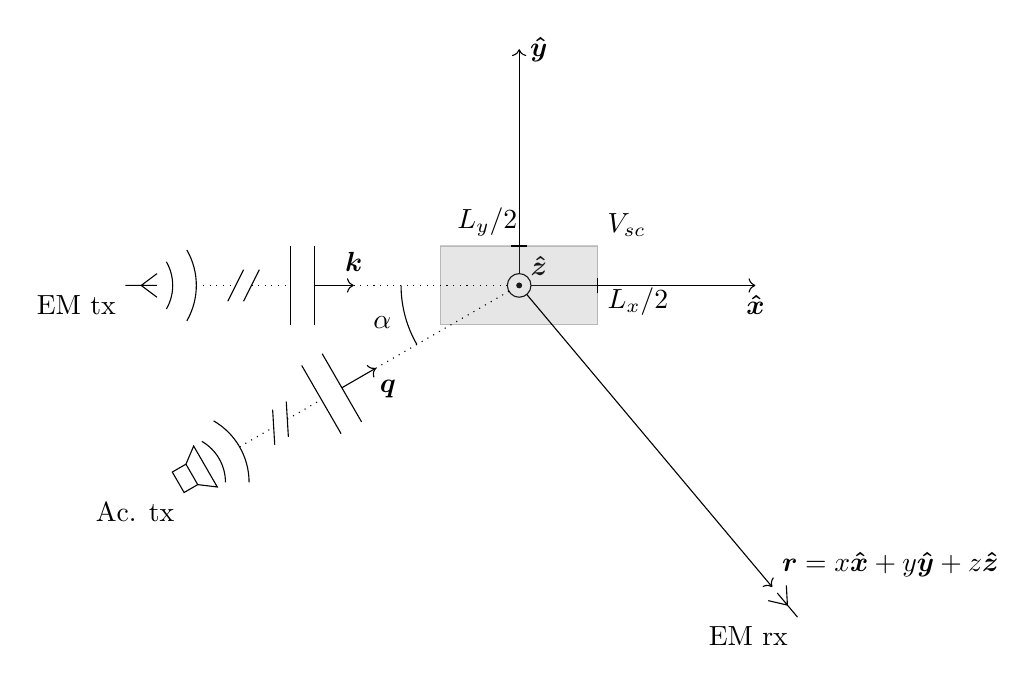
\begin{tikzpicture}
			% Draw coordinate axes
			\draw (0,0) circle(0.15);
			\filldraw[black] circle(0.03);
			\draw[->] (0.15,0) -- (3,0);
			\draw[->] (0,.150) -- (0,3);
			\draw (3,-0.25) node{$\bm{\hat{x}}$} (0.25,3) node{$\bm{\hat{y}}$} (0.25,0.25) node{$\bm{\hat{z}}$};
			
			% Draw scattering cube (or rectangle in this case)
			\draw[fill=gray,opacity=0.2] (-1,-0.5) rectangle(1,0.5);
			\draw (1,-0.1) -- (1,0.1) node[anchor= north west]{$L_{x}/2$} (-0.1,0.5) -- (0.1,0.5) node[anchor= south east]{$L_{y}/2$} (1,0.5) node[anchor=south west]{$V_\mrm{sc}$};
			
			% Draw EM tx and spherical waves
			\draw[shift = {(-5,0)}] (0,0) node[anchor=north east]{EM tx} -- (0.4,0) (0.2,0) -- (0.4,0.15)
			(0.2,0) -- (0.4,-0.15);
			\draw[shift = {(-5,0)}] ([shift={(-30:0.6)}] 0,0) arc(-30:30:0.6) ([shift={(-30:0.9)}] 0,0) arc(-30:30:0.9);
			
			% Draw EM "long distance" lines
			\draw[shift = {(-4.1,0)},dotted] (0,0) -- (0.5,0) (0.7,0) -- (1.2,0);
			\draw[shift = {(-4.1,0)}] (0.4,-0.2) -- (0.6,0.2) (0.6,-0.2) -- (0.8,0.2);
			
			% Draw EM plane waves
			\draw[shift = {(-2.9,0)}] (0,-0.5) -- (0,0.5) (0.3,-0.5) -- (0.3,0.5);
			\draw[shift = {(-2.6,0)}, ->] (0,0) -- (0.5,0);
			\draw[shift = {(-2.6,0)}] (0.5,0.3) node{$\bm{k}$};
			\draw[dotted] (-0.15,0) -- (-2.1,0);
			
			% Draw Ac. tx and spherical waves
			\draw[shift = {(210:5)}, rotate = 30] (0,-0.15) node[anchor=north east]{Ac. tx} rectangle (0.2,0.15) -- (0.4,0.3) -- (0.4,-0.3) -- (0.2,-0.15);
			\draw[shift = {(210:5)}, rotate = 30] ([shift={(-30:0.6)}] 0,0) arc(-30:30:0.6) ([shift={(-30:0.9)}] 0,0) arc(-30:30:0.9);
			
			% Draw Ac. "long distance" lines
			\draw[shift = {(210:4.1)}, rotate = 30,dotted] (0,0) -- (0.5,0) (0.7,0) -- (1.2,0);
			\draw[shift = {(210:4.1)}, rotate = 30] (0.4,-0.2) -- (0.6,0.2) (0.6,-0.2) -- (0.8,0.2);
			
			% Draw Ac. plane waves
			\draw[shift = {(210:2.9)}, rotate = 30] (0,-0.5) -- (0,0.5) (0.3,-0.5) -- (0.3,0.5);
			\draw[shift = {(210:2.6)}, rotate = 30, ->] (0,0) -- (0.5,0);
			\draw[shift = {(210:2.6)}, rotate = 30] (0.5,-0.3) node{$\bm{q}$};
			\draw[rotate = 30, dotted] (-0.15,0) -- (-2.1,0);
			
			% Draw angle alpha
			\draw ([shift={(180:1.5)}] 0,0) arc(180:210:1.5) (195:1.8) node{$\alpha$};
			
			% Draw line towards receiver
			\draw[->] (310:0.15) -- (310:5) node[anchor=south west]{$\bm{r} = x\bm{\hat{x}} + y\bm{\hat{y}} + z\bm{\hat{z}}$};
			
			% Draw EM rx
			\draw[shift = {(310:5.5)}, rotate = 130] (0,0) node[anchor=north east]{EM rx} -- (0.4,0) (0.2,0) -- (0.4,0.15) (0.2,0) -- (0.4,-0.15);
		\end{tikzpicture}
		}
		\caption{\label{fig:radareq-geom-main} Geometry for the scattering problem.}
	\end{figure}
	The $xy$-plane is defined as the plane formed by the acoustic and electromagnetic wavevectors (they are assumed to be non-parallel). The scattering volume is a cuboid with dimensions $L_x$, $L_y$ and $L_z$. It is centered in the origin of the coordinate system, and both the acoustic and electromagnetic waves are approximated as plane waves close to the origin. Thus, the electromagnetic and dielectric perturbation fields near the origin are defined as
	\begin{align}
		\bm{E}_i (\bm{r}',t) &= \bm{E}_i (\bm{r}') = \bm{E}_{i0} e^{i\bm{k}\cdot\bm{r}'} \label{eq:an-radar-planeE} \\
		\varepsilon_1 (\bm{r}',t) &= -\mathfrak{p} \varepsilon_r^2 s_p \cos(\bm{q} \cdot \bm{r}' - \Omega t) \label{eq:an-radar-planeEps}
	\end{align}
	Here, $\bm{E}_{i0}$ is the complex field amplitude at the origin ($-i\omega t$ time-dependence separated) and $\bm{k}$ is the electromagnetic wavevector. A scalar photoelastic relation has been assumed, where $\mathfrak{p}$ is the photoelastic constant, $S_0$ is the acoustic strain amplitude at the origin, $\bm{q}$ is the acoustic wavevector and $\Omega$ the acoustic frequency.
	
	For simplicity, the electromagnetic polarization is assumed to be in z, $\bm{E}_{i0} \parallel \bm{\hat{z}}$. This is also in part done to avoid polarization changes in the scattered field \cite{Korpel1988}. Due to this $\nabla(\bm{E}_i \cdot \nabla \varepsilon_1) = \bm{0}$ which simplifies the scattering integral to
	\begin{equation*}
		\bm{E}_{sc}(\bm{r},t) = \frac{k^2}{4\pi\varepsilon_r} \int_{V_{sc}} \frac{e^{ik |\bm{r}-\bm{r'}| }}{ |\bm{r}-\bm{r'}|} \bm{E}_i (\bm{r'},t) \varepsilon_1 (\bm{r'},t) \mathrm{d}v'
	\end{equation*}
	Equation \eqref{eq:an-radar-planeE} and \eqref{eq:an-radar-planeEps} are now inserted, and with a far-field approximation and expansion of the cosine as complex exponentials the integral is written as
	\begin{equation*}
	\begin{split}
		\bm{E}_{sc}(\bm{r},t) =& -\frac{\varepsilon_rk^2 e^{ikr}}{8\pi r} \bm{E}_{i0} \mathfrak{p} s_p \\
		&\cdot \left( e^{-i\Omega t} \int_{V_{sc}} e^{i( k(\bm{\hat{k}} - \bm{\hat{r}}) + \bm{q} ) \cdot \bm{r}'} \mathrm{d}v + e^{i\Omega t} \int_{V_{sc}} e^{i( k(\bm{\hat{k}} - \bm{\hat{r}}) - \bm{q} ) \cdot \bm{r}'} \mathrm{d}v' \right)
	\end{split}
	\end{equation*}
	The solution to this integral is written as (see \ref{sec:app-derivations-radar})
	\begin{equation*}
		\bm{E}_{sc} (\bm{r},t) = -\bm{E}_{i0} \left( E_A^+ (\bm{r},t) + E_A^- (\bm{r},t) \right)
	\end{equation*}
	where
	\begin{equation*}
		E_A^\pm (\bm{r},t) = \frac{\varepsilon_rk^2 e^{ikr}}{8\pi r} \mathfrak{p} s_p L_x L_y L_z e^{\mp i\Omega t} \Phi^\pm (\theta,\phi)
	\end{equation*}
	and
	\begin{equation*}
	\begin{split}
		\Phi^\pm(\theta,\phi) =& \text{sinc} \left( \frac{L_x}{2\pi} \left( k - k\sin{\theta}\cos{\phi} \pm q\cos{\alpha} \right) \right) \\
		\cdot& \text{sinc} \left( \frac{L_y}{2\pi} \left( -k\sin{\theta}\sin{\phi} \pm q\sin{\alpha} \right) \right) \\
		\cdot& \text{sinc} \left( -\frac{L_z}{2\pi} k\cos{\theta} \right)
	\end{split}
	\end{equation*}
	One important detail to note is that two distinct frequency components arise: one where the frequency is shifted up by $\Omega$ ($E_A^+$) and one where it is shifted down by $\Omega$ ($E_A^-$).
	
	To obtain a more practical expression, the equations are now transformed into power. The time average on the short time-scale ($\omega$, not $\Omega$) of the Poynting vector is \cite{Kristensson2008}
	\begin{equation*}
	\left< \bm{S}_{sc} \right> = \frac{1}{2} \mathrm{Re}\left\{ \bm{E}_{sc} \times \bm{H}_{sc}^* \right\}
	\end{equation*}
	where the E- and H-fields are complex with long time-scale time dependence. The magnetic field $\bm{H}_{sc}$ is given by \cite{Kristensson2008}
	\begin{equation*}
	\bm{H}_{sc} \approx \frac{1}{ik \eta_0 \eta} \nabla \times \bm{E}_{sc}
	\end{equation*}
	where $\eta_0$ is the wave impedance of free space and $\eta_0 \eta$ the wave impedance in the material. The scattered electric field is inserted, and in the far-field the cross product can then be calculated to be
	\begin{equation*}
	\bm{E}_{sc} \times \bm{H}_{sc}^* = \frac{\bm{\hat{r}}}{\eta_0 \eta} |\bm{E}_{i0}|^2 |E_A (\bm{r},t)|^2
	\end{equation*}
	The time-averaged Poynting vector is now calculated as
	\begin{equation*}
	\left< \bm{S}_{sc} \right> = \frac{1}{2}\mathrm{Re}\left\{ \bm{E}_{sc} \times \bm{H}_{sc}^* \right\} = \frac{\bm{\hat{r}}}{2\eta_0 \eta} |\bm{E}_{i0}|^2 |E_A (\bm{r},t)|^2
	\end{equation*}
	If the two frequency components are now considered individually,
	\begin{equation*}
		|E_A^\pm (\bm{r},t)|^2 =\frac{\varepsilon_r^2 k^4}{64 \pi^2 r^2} \mathfrak{p}^2 s_p^2 L_x^2 L_y^2 L_z^2 \Phi^\pm (\theta,\phi)^2
	\end{equation*}
	
	Using standard antenna parameters, the incident field can be written as
	\begin{equation*}
		|\bm{E}_{i0}|^2 = 2\eta_0 \eta \frac{P_T G_T}{4\pi R_T^2}
	\end{equation*}
	where $P_T$ is the power accepted by the antenna, $G_T$ is the maximum gain of the antenna and $R_T$ is the distance from the antenna to the scattering center. This is inserted into the time-average of the power density, giving
	\begin{equation*}
		\left< \bm{S}_{sc} \right>^\pm = \bm{\hat{r}} \frac{P_T G_T}{4\pi R_T^2} \frac{\varepsilon_r^2 k^4}{64 \pi^2 r^2} \mathfrak{p}^2 s_p^2 L_x^2 L_y^2 L_z^2 \Phi^\pm (\theta,\phi)^2
	\end{equation*}
	
	Now the effects of the receiving antenna are considered. It is assumed that this antenna is optimally directed towards the scattering center. The received power is then
	\begin{equation*}
		P_R^\pm = \left| \left< \bm{S}_{sc} \right>^\pm \right| A_e
	\end{equation*}
	where $A_e$ is the effective area of the antenna, which can be rewritten as
	\begin{equation*}
		A_e = \frac{\lambda_R^2 G_R}{4\pi}
	\end{equation*}
	where $G_R$ is the gain of the receiving antenna. $\lambda_R$ should be the wavelength at the antenna here, which is not necessarily the same as in the material. Combining this with earlier results gives a received power of
	\begin{equation*}
		P_R^\pm = \frac{\lambda_R^2 G_R}{4\pi} \frac{P_T G_T}{4\pi R_T^2} \frac{\varepsilon_r^2 k^4}{64 \pi^2 R_R^2} \mathfrak{p}^2 s_p^2 L_x^2 L_y^2 L_z^2 \Phi^\pm (\theta,\phi)^2
	\end{equation*}
	where $R_R$ is the distance between the scattering center and the receiver, and the receiver is located in the direction $(\theta,\phi)$ as seen from the scattering center. For a more traditional bistatic radar equation this can be written as
	\begin{equation*}
		P_R^\pm = \frac{P_T G_T G_R \lambda_R^2 \sigma^\pm (\theta,\phi)}{(4\pi)^3 R_T^2 R_R^2}
	\end{equation*}
	with the radar cross-section given by
	\begin{equation*}
		\sigma^\pm (\theta, \phi) = \frac{\varepsilon_r^2 k^4}{16\pi} \mathfrak{p}^2 s_p^2 L_x^2 L_y^2 L_z^2 \Phi^\pm (\theta,\phi)^2
	\end{equation*}
	
	When actually measuring a signal, signal-to-noise ratio (SNR) is a more practical quantity than received power. The equation can be rewritten using SNR (see appendix \ref{app:derivations}) as:
	\begin{equation*}
		\textit{SNR}^\pm_N = \frac{P_T G_T G_R \lambda_R^2 \sigma^\pm (\theta,\phi)}{(4\pi)^3 R_T^2 R_R^2 k_B T_0 B F} N
	\end{equation*}
	where $k_B$ is Boltzmann's constant, $T_0$ is the standard temperature 290 K, $B$ is the receiver bandwidth, $F$ is the noise ratio of the receiver and $N$ is the number of samples recorded. This equation assumes that coherent demodulation and integration is used to boost the SNR.
	
	Inspection of the equations for either scattered power or SNR shows that all geometry dependence is contained in the function $\Phi^\pm$. This depends on the observation angles $\theta$, $\phi$ and the angle between EM and Ac. wavevectors $\alpha$. Conditions for the angles maximizing scattering are derived in \ref{sec:app-derivations-bragg} and can be summarized as:
	\begin{align}
		\theta &= \pi/2 \label{eq:an-bragg-theta} \\
		\cos{\alpha} = \mp \frac{q}{2k} &= \mp \frac{\lambda}{2\Lambda} \label{eq:an-bragg-alpha} \\
		\phi &= \mp \pi + 2\alpha \label{eq:an-bragg-phi}
	\end{align}
	The $\mp$-sign here is related to the $\pm$-sign indicating frequency shift of the scattered wave. These equations correspond directly to the Bragg condition used in acousto-optics (see \ref{sec:app-derivations-bragg} for derivation). This gives the model some validation since the acousto-optic Bragg condition is derived from a slightly different starting point, but for the same basic phenomenon \cite{Saleh2007}.
	
	\todoext{I have a new derivation which is based on a parallelogram interaction region (still based on plane waves, but uses beam widths to define the interaction region). This could be added here to show the result of another interaction region.}
	
	\chapter{Numerical Simulation}
	
	\section{Overview}
	\todoint[inline]{Description of how different basic things (such as antennas and transducers) are modeled. Details on COMSOL and other similar stuff.}
	The problem was simulated in COMSOL Multiphysics for verification and further investigation of more complex scenarios than the one modeled analytically. The two physics interfaces used were the "Pressure Acoustics, Frequency Domain" from the basic COMSOL Multiphysics and "Electromagnetic Waves, Frequency Domain" from the RF Module.
	
	\todoint[inline]{Describe why the frequency shift is not visible, and why this is not possible with the particular simulations used}
	
	\subsection{Tapering of apertures}
	To reduce sidelobe levels, both the electromagnetic and acoustic apertures had amplitude tapers applied to them. \addref This had the effect of lowering the electric field or acoustic acceleration near the edges of apertures. The specific taper used was a Gaussian taper, which multiplies values at the aperture with a Gaussian function given by
	\begin{equation*}
	e^{-(Ay')^2}
	\end{equation*}
	where $A$ affects the width of the taper and $y'$ is a coordinate along the aperture with 0 in the center. Since the model was based on a circle and all apertures were modeled as straight lines on the edge of the circle, $y'$ can be found by rotation of the original coordinate $y$ by the angle $\phi$. This transformation is given by \addref
	\begin{equation*}
		\begin{bmatrix}
			x' \\
			y'
		\end{bmatrix}
		=
		\begin{bmatrix}
			\cos{\phi} & \sin{\phi} \\
			-\sin{\phi} & \cos{\phi}
		\end{bmatrix}
		\begin{bmatrix}
			x \\
			y
		\end{bmatrix}
	\end{equation*}
	which gives the equation for $y'$
	\begin{equation*}
		y' = -x\sin{\phi} + y\cos{\phi}
	\end{equation*}
	The geometry is the same as previously shown in figure \ref{fig:radareq-geom-main}. As such, $\phi = \pi$ for EM and $\phi = \pi + \alpha$ for Ac. For the coefficient $A$, it was found that $A = 4/d_a$ gave a good taper for an aperture length $d_a$.
	
	\subsection{Modeling of Electromagnetic Antenna}
	An electromagnetic antenna was modeled using the "Port" boundary condition with options "User Defined" and wave excitation turned on. The port input power was set to 15 dBm. Due to it being located on an interior boundary, the slit condition was activated with a domain-backed slit. For the port mode, the electric field was set as the input quantity with a tapered field in z defined as
	\begin{equation*}
		E_{0z} = e^{-(4y/d_a)^2}
	\end{equation*}
	where $y$ is a coordinate and $d_a$ the aperture length. The propagation constant was set to the wave number in the material using "emw.k".
	
	\subsection{Modeling of Ultrasonic Transducer}
	An ultrasonic transducer was modeled using the "Normal Acceleration" boundary condition. The acceleration was set to "Inward acceleration". The value of the acceleration amplitude was calculated from a displacement amplitude using $a_0 = \Omega^2 u_p$ where the displacement amplitude is the same as described in the theory. The acceleration was tapered as
	\begin{equation*}
		a_n = a_0 e^{-(4(x\sin{\alpha} - y\cos{\alpha})/d_a)^2}
	\end{equation*}
	where $x$ and $y$ are coordinates and $d_a$ the aperture length.
	
	\subsection{Photoelasticity model}
	To model photoelasticity in COMSOL, equation \eqref{eq:th-PE-scalar-p} was used with the photoelastic constant defined by equation \eqref{eq:th-PE-liquid-model}.
	
	\subsection{Geometry and boundary conditions}
	The basic geometry is shown in figure \ref{fig:sim-geometry} for the acoustic and electromagnetic simulations. The only difference in geometry between the two is the Perfectly Matched Layer (PML) which is used in the electromagnetic simulation but not the acoustic simulation. Additionally, the boundary conditions are different for the two simulations which is also shown. One boundary of special interest is the "Measurement boundary". This is where the physics domain ends, and the fields were measured at this boundary for post-processing.
	
	The PML was used to emulate an open boundary at the measurement boundary for the electromagnetic problem. It was a cylindrical type with center in the center of the geometry and a width of $2\lambda$. It used polynomial coordinate stretching with a typical wavelength taken from the electromagnetic physics interface. The PML scaling factor and PML scaling curvature parameter were both set to 1. At the exterior boundary, a Perfect Electric Conductor (PEC) boundary condition was used.
	
	The PML function was not available for the basic pressure acoustics interface used here. However, the Cylindrical Wave Radiation boundary condition was available and was used for the same purpose as a PML.
	
	\begin{figure}
		\centering
		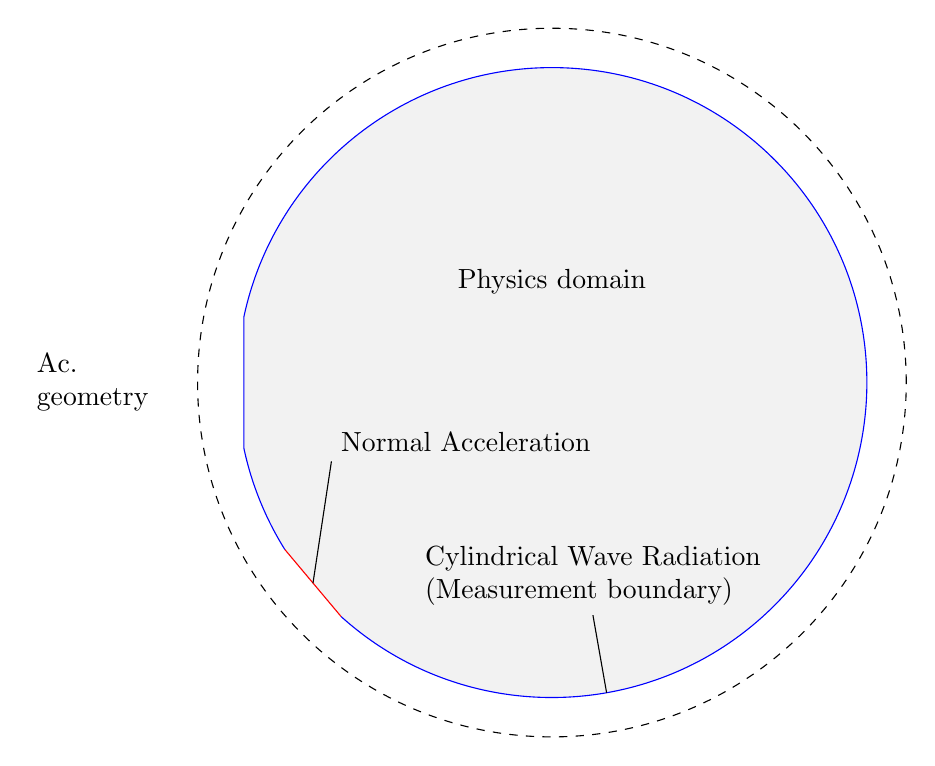
\begin{tikzpicture}
	
	% Fill domain
	\fill[gray!10] (0:4) arc(0:180-12:4) -- (180+12:4) arc(180+12:220-8:4) -- (220+8:4) arc(220+8:360:4);
	
	% Draw port
	\draw[red] (220-8:4) -- (220+8:4);
	
	% Draw inner boundary
	\draw[blue] (0:4) arc(0:180-12:4) -- (180+12:4) arc(180+12:220-8:4) (220+8:4) arc(220+8:360:4);
	
	% Draw outer boundary
	\draw[dashed] (0,0) circle(4.5);
	
	% Label domains
	\draw (0,1) node[anchor=south] {Physics domain};
	
	% Label boundaries
	\draw (220:{4*cos(8)}) -- (-2.8,-1) node[anchor=south west] {Normal Acceleration};
	\draw (280:4) -- (280:3) node[anchor=south, align=left] {Cylindrical Wave Radiation\\(Measurement boundary)};
	
	% Ac label
	\draw (180:5) node[anchor=east, align=left] {Ac.\\geometry};
	
\end{tikzpicture}
		\vspace{5 mm}
		
		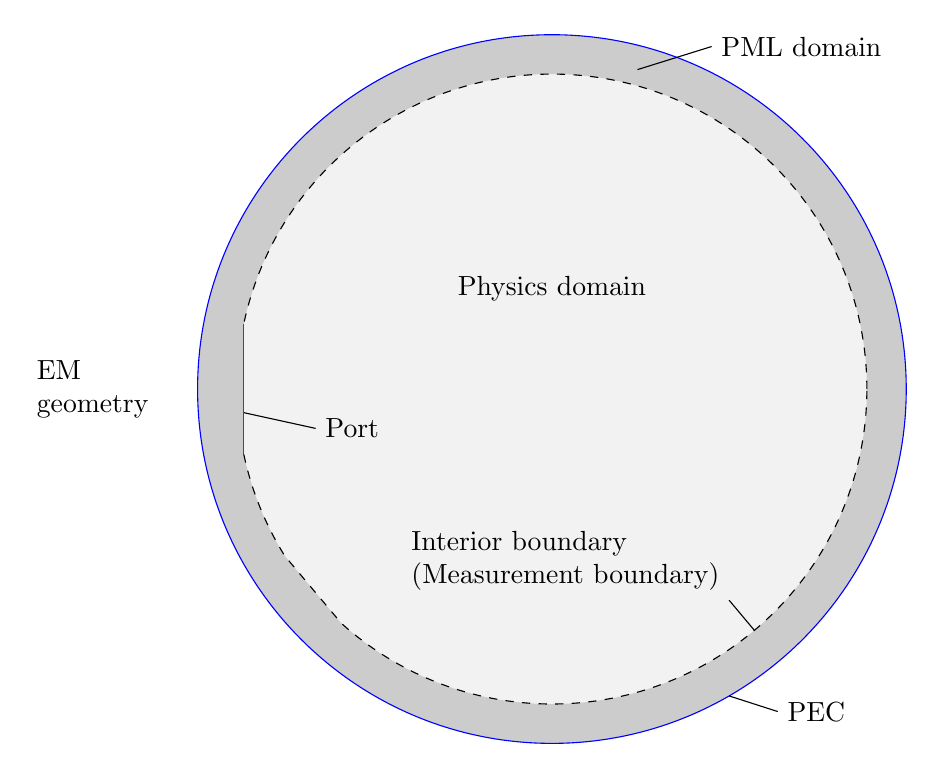
\begin{tikzpicture}
	
	% Fill domain
	\fill[gray!10] (0:4) arc(0:180-12:4) -- (180+12:4) arc(180+12:220-8:4) -- (220+8:4) arc(220+8:360:4);
	
	% Draw PML
	\fill[fill=gray!40, even odd rule] (0,0) circle(4.5) (0:4) arc(0:180-12:4) -- (180+12:4) arc(180+12:220-8:4) -- (220+8:4) arc(220+8:360:4);
	
	% Draw port
	\draw[red] (180-12:4) -- (180+12:4);
	
	% Draw inner boundary
	\draw[dashed] (0:4) arc(0:180-12:4) (180+12:4) arc(180+12:220-8:4) -- (220+8:4) arc(220+8:360:4);
	
	% Draw outer boundary
	\draw[blue] (0,0) circle(4.5);
	
	% Label domains
	\draw (0,1) node[anchor=south] {Physics domain};
	\draw (75:4.2) -- (65:4.8) node[anchor=west] {PML domain};
	
	% Label boundaries
	\draw (-60:4.5) -- (-55:5) node[anchor=west, align=left] {PEC};
	\draw (-{4*cos(12)},-0.3) -- (-3,-0.5) node[anchor=west] {Port};
	\draw (310:4) -- (310:3.5) node[anchor=south east, align=left] {Interior boundary\\(Measurement boundary)};
	
	% EM label
	\draw (180:5) node[anchor=east, align=left] {EM\\geometry};
	
\end{tikzpicture}
		\caption{\label{fig:sim-geometry} Simulation geometry with boundary conditions for Ac. and EM simulations.}
	\end{figure}
	
	\subsection{Material}
	The material model used was based on a foam core. The reason for this was that foam material is fairly homogeneous and isotropic (compared to honeycombs) and is used in aerospace applications \addref. The specific core selected was Divinycell HT251 from Diab Group, which is an aerospace core with applications described as "Primary structures, radomes, control surfaces and interior components" \cite{Diab2016}. The relevant material properties were density ($\rho_0$), bulk modulus ($K$) and relative permittivity ($\varepsilon_r$). These were $\rho_0 = 250$ kg/m$^3$, $K = 400$ MPa (nominal) and $\varepsilon_r = 1.29$ \cite{Diab2016}. In COMSOL, the required properties were density, speed of sound, relative permittivity, relative permeability and electric conductivity \todoint{More properties?}. The speed of sound was calculated using $v = \sqrt{K/\rho_0}$ \todoint{reference equation}, the relative permeability was set to 1 and the conductivity to 0. The assumption was that the material was perfectly non-conducting and non-magnetic.
	
	\subsection{Mesh}
	Two meshes were used in simulations: one for the acoustic simulation and one for the electromagnetic simulation. The reason for this was primarily the difference in wavelength.
	
	The acoustic mesh was defined on both the physics domain and PML domain even though only the physics domain was simulated in this case. A free triangular mesh was used with element size between $\Lambda/10$ and $\Lambda/10 \cdot 3 \cdot 10^{-2}$ in the physics domain, and "Fine" in the PML domain. Before running the free triangular meshing, the mesh was defined on the measurement boundary.
	
	The electromagnetic mesh used a free triangular mesh in the physics domain and a mapped mesh in the PML domain. The element size in the physics domain was between $\lambda/10$ and $\lambda/10 \cdot 3 \cdot 10^{-2}$. Before running the free triangular meshing, the mesh was defined on the measurement boundary.
	
	\subsection{Simulation studies}
	Before starting simulations, the frequencies, material and geometry were defined. The geometry was in many parts defined as a function of the frequencies and material properties in order to obtain reasonably sized domains and apertures placed according to the Bragg condition.
	
	For the actual simulations, the work flow is illustrated in figure \ref{fig:simulationflow}. First, an acoustic frequency domain study was run using the acoustic frequency and mesh. The result from this was a complex pressure field. Real part convention was used when relating this complex field to the actual pressure.
	
	To transform the pressure to relative permittivity, a variable was used in the material model to define the relative permittivity. This variable took the real part of the pressure field as its input, and used equations \eqref{eq:th-PE-scalar} and \eqref{eq:th-PE-scalar-p} to calculate a corresponding field for $\varepsilon_1$.
	
	An electromagnetic frequency domain study was now run using the electromagnetic frequency and mesh. The acoustic study was used for calculating initial values for variables not solved for. This was necessary for the pressure field to be available in both studies. Since the photoelastic effect is usually very small, the scattered field was not possible to distinguish with the incident field present. To be able to isolate the scattered field, two simulations were run: one where the relative permittivity of the material was unperturbed and one where it was perturbed by $\varepsilon_1$. The difference between fields resulting from these simulations were identified as the scattered fields.
	
	Due to limitations in the post-processing capabilities of COMSOL, the $E_z$, $H_x$ and $H_y$ fields at the boundary were exported together with $x$ and $y$ coordinates after the electromagnetic simulation was finished. This was done both for the simulation with and without perturbation.
	
	\begin{figure}[h]
		\centering
		\resizebox{\textwidth}{!}{
			
% http://www.texample.net/tikz/examples/simple-flow-chart/
\tikzstyle{sim} = [rectangle, draw, fill=blue!20, 
text width=5em, text centered, rounded corners, minimum height=4em]
\tikzstyle{res} = [draw, ellipse,fill=red!20]

\begin{tikzpicture}[node distance = 2 cm, auto]

	\draw[dashed] (-2,1) rectangle(2,-7);
	\node[anchor=south west, text width=10em] at (-2,1) {Pressure acoustics, frequency domain};
	
	\node[sim] at (0,0) (Ac) {Ac. Simulation};
	\node[res, below of=Ac] (p) {$p$ field};
	\node[sim, below of=p] (real) {Calculation on real part};
	\node[res, below of=real] (er) {$\varepsilon_1$ field};
	
	\draw[->] (Ac) -- (p);
	\draw[->] (p) -- (real);
	\draw[->] (real) -- (er);
	
	\draw[dashed] (4,1) rectangle(12,-3);
	\node[anchor=south west, text width=11em] at (4,1) {Electromagnetic waves, frequency domain};
	
	\node[sim] at (6,0) (EM1) {EM Simulation w/o PE};
	\node[res, below of=EM1] (emw1) {$\bm{E}_i$, $\bm{H}_i$ fields};
	\node[sim] at (10,0) (EM2) {EM Simulation w/ PE};
	\node[res, below of=EM2] (emw2) {$\bm{E}$, $\bm{H}$ fields};
	
	\draw[->] (EM1) -- (emw1);
	\draw[->] (EM2) -- (emw2);
	
	\draw[->] (er.east) -- (3,-6) -- (3,2.5) -- (10,2.5) -- (EM2.north);
	
	\node[sim] at (8,-4) (diff) {Difference};
	\node[res, below of=diff] (sc) {$\bm{E}_{sc}$, $\bm{H}_{sc}$ fields};
	\draw[->] (emw1.south) -- (6,-4) -- (diff.west);
	\draw[->] (emw2.south) -- (10,-4) -- (diff.east);
	\draw[->] (diff.south) -- (sc.north);
	
\end{tikzpicture}
		}
		\caption{\label{fig:simulationflow} Simulation flow chart}
	\end{figure}
	
	\subsection{Post-processing}
	The simulation results were further processed in SciPy for better visualization of the results than what was possible in COMSOL. The $E_z$, $H_x$ and $H_y$ fields (both with and without photoelastic perturbation) on the domain boundary were exported from COMSOL and loaded in SciPy. The differences between the fields were calculated to obtain the scattered fields. The time-averaged Poynting vector was then calculated as
	\begin{align*}
	\left< S_x \right> &= -\frac{1}{2} \text{Re} \{ E_z H_y^* \} \\
	\left< S_y \right> &= \frac{1}{2} \text{Re} \{ E_z H_x^* \}
	\end{align*}
	Due to it being easier to visualize, the magnitude of the time-averaged Poynting vector was also calculated. Using the $x$ and $y$ coordinates, the observation angle $\phi_{obs}$ for each point was calculated and the data was sorted according to this. A measure for the total scattered power was calculated by integrating the magnitude of the time-averaged Poynting vector over the entire boundary. This was done using the trapezoidal method with the distances between points calculated from the coordinates.
	
	One thing to note is that the definition for radiated power is
	\begin{equation*}
		\int_S \left< \bm{S} \right> \cdot \bm{\hat{n}} \, dS
	\end{equation*}
	where $\bm{\hat{n}}$ is the normal to the surface. However, here the calculation was instead
	\begin{equation*}
		\int_S \left| \left< \bm{S} \right> \right|  \, dS
	\end{equation*}
	The reason behind this is that the boundary curvature was large when compared with the beams of interest. This would cause scattered field originating away from the center of the geometry to have less influence on the measure for total scattered power. This can be seen in figure \ref{fig:sim-postproc-angles} where the propagation angle, $\phi_{prop}$, differs from the observation angle normal to the boundary, $\phi_{obs}$, for much of the scattered field. Using the magnitude of the Poynting vector instead decreases the influence of the boundary geometry.
	
	For plotting of the time-averaged Poynting vector magnitude, the propagation angle $\phi_{prop}$ was calculated for each data point. The two angles $\phi_{obs}$ and $\phi_{prop}$ are shown in figure \ref{fig:sim-postproc-angles} together with the geometry of the problem. From this figure it can be seen that the observation angle depends highly on the measurement point while the propagation angle is a property of the scattered field. For this reason, the propagation angle was chosen for use in plots where the angle mattered.
	
	\begin{figure}[h]
		\centering
		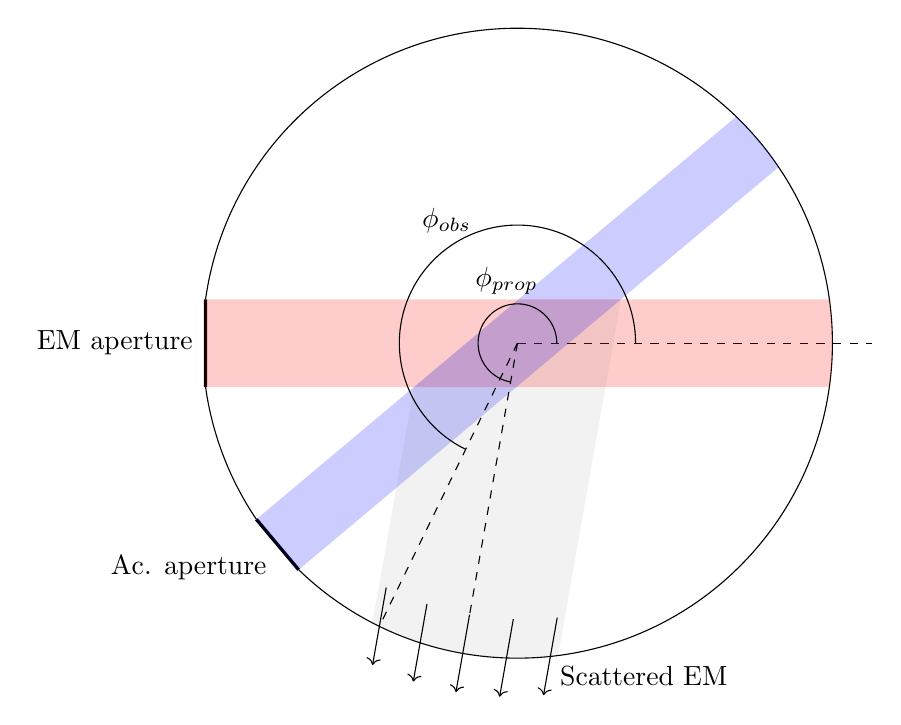
\begin{tikzpicture}
	% Draw coordinate lines (dashed)
	\draw[dashed] (0,0) -- (4.5,0);
	
	% Draw boundary
	\draw (0:4) arc(0:172:4) (188:4) arc(188:214:4) (226:4) arc(226:360:4);
	\draw[very thick] (172:4) -- (188:4) (214:4) -- (226:4);
	
	% Draw incident beams
	\fill[red,opacity=0.2] (172:4) -- (8:4) arc(8:-8:4) -- (188:4) -- cycle;
	\fill[blue,opacity=0.2] (214:4) -- (46:4) arc(46:34:4) -- (226:4) -- cycle;
	
	% Find intersections for interaction region definition
	\draw (172:4) coordinate(em1a) (8:4) coordinate(em1b) (188:4) coordinate(em2a) (-8:4) coordinate(em2b);
	\draw (214:4) coordinate(ac1a) (46:4) coordinate(ac1b) (226:4) coordinate(ac2a) (34:4) coordinate(ac2b);
	\coordinate (c1) at (intersection of em2a--em2b and ac1a--ac1b);
	\coordinate (c2) at (intersection of em1a--em1b and ac1a--ac1b);
	\coordinate (c3) at (intersection of em1a--em1b and ac2a--ac2b);
	
	% Draw scattered beam
	\begin{scope}
		\clip (0,0) circle(4);
		\fill[gray,opacity=0.1] (c1) -- (c2) -- (c3) -- ([shift={(c3)}] 260:6) -- ([shift={(c1)}] 260:6) -- cycle;
	\end{scope}
	
	% Draw field vectors
	\draw[->, shift={(260:4)}, rotate=260] (-0.5,0) -- (0.5,0);
	\draw[->, shift={(268:4)}, rotate=260] (-0.5,0) -- (0.5,0);
	\draw[->, shift={(276:4)}, rotate=260] (-0.5,0) -- (0.5,0);
	\draw[->, shift={(252:4)}, rotate=260] (-0.5,0) -- (0.5,0);
	\draw[->, shift={(244:4)}, rotate=260] (-0.5,0) -- (0.5,0);
	
	% Draw lines from origin to vectors
	\draw[dashed] (260:0) -- (260:3.5);
	\draw[dashed] (0,0) -- ([shift={(244:4)}, rotate=260] 0,0);
	
	% Draw angles
	\draw ([shift={(0:0.5)}] 0,0) arc(0:260:0.5) (100:0.8) node{$\phi_\mrm{prop}$};
	\draw ([shift={(0:1.5)}] 0,0) arc(0:244:1.5) (120:1.8) node{$\phi_\mrm{obs}$};
	
	% Descriptions for beams
	\draw (180:4) node[anchor=east] {EM aperture};
	\draw (220:4) node[anchor=north east] {Ac. aperture};
	\draw (276:4) node[anchor=north west] {Scattered EM};
	
\end{tikzpicture}
		\caption{\label{fig:sim-postproc-angles} Propagation and observation angle near the edge of the scattered beam.}
	\end{figure}
		
	\section{Verification of analytical model}
	\todoext{Description of how the simple scattering problem was modeled.}
	To verify the results from section \ref{sec:analytical-radar} the frequencies of the acoustic and electromagnetic waves were matched to a Bragg angle of $40^\circ$ while the angle $\alpha$ between the wavevectors was swept between $\pm 5^\circ$ of the optimal angle. This was done both for (+) and (-) scattering by sweeping around either $\alpha = 40^\circ$ or $\alpha = 120^\circ$, as these angles are the ones given by equation \eqref{eq:an-bragg-alpha} as angles for maximum scattering.
	
	\section{Effect of voids}
	\todoext{Description of how voids were modeled. Relate to delaminations.}
	
	\section{Effect of conductive defects}
	To examine the effect of a defect with electromagnetic contrast but no acoustic contrast, simulations were run with a conductive defect. The geometry of this problem was based on the basic geometry shown in figure \ref{fig:sim-geometry}. The addition was a circle in the center of the physics domain representing a defect. This had the diameter equal to the electromagnetic wavelength $\lambda$. The material in this region was the same as in the physics domain, but with a nonzero electric conductivity.
	
	To demonstrate the effect of conductivity, the electric conductivity of the defect was swept between 0 and 10 S/m.
	
	\chapter{Results and Discussion}
	\todoext{It might be better to have results and discussion separated?}
	
	\section{Numerical Simulation Results}
	
	\subsection{Verification of analytical model}
	\todoint[inline]{Comparison of results from the simulation with the analytical model. Primarily a verification of the Bragg condition, but maybe also some comparison of the power levels.}
	
	\subsection{Effect of voids}
	
	\section{Effect of conductive defects}
	
	\section{Possibilities for NDT}
	
	\section{Future Work}
	\todoext{More detailed simulations - accurate modeling of the EM antenna, Ac. transducer, propagation from outside into the sample etc. Would require simulation of elastic waves in addition to acoustic waves. Possible in COMSOL if the acoustics module and structural mechanics module are used (those were not available to me). The improved acoustics simulation would enable investigation of things such as s-waves, transducer coupling etc.}
	
	\todoext{Experiments - simple verification of the photoelastic interaction mechanism at the specific combination of ultrasound/microwave or ultrasound/mm-wave frequencies. Primarily, the Bragg condition would be the most interesting thing to verify. Both the angle and frequency requirements and shifts are interesting.}
	
	\section{Conclusion}
	
	
	\bibliographystyle{../../Litteratur/IEEEtran}
	\bibliography{../../Litteratur/litteratur}
	
	\appendix
	
	\chapter{Appendix: Full Derivations \label{app:derivations}}
	
	\section{Derivation of scattering integral for perturbed dielectrics \label{sec:app-derivations-scatter}}
	Here follows a formal derivation of the scattering of electromagnetic waves against a perturbation in relative permittivity. This is useful in photoelastic interaction since an acoustic wave in that case causes a periodic dielectric perturbation. Most of this derivation is based on a similar derivation by Tatarskii which considers scattering from turbulence in air \cite{Tatarskii1971}.
	
	\subsection{General equation for electric field in perturbated dielectric}
	First, Maxwell's equations for a linear, non-magnetic, source-free, isotropic dielectric are presented. Note that the permittivity is not homogeneous.
	\begin{align*}
		&\nabla \times \bm{\mathcal{E}} = -\mu_0 \frac{\partial \bm{\mathcal{H}}}{\partial t} \\
		&\nabla \times \bm{\mathcal{H}} = \frac{\partial (\varepsilon \bm{\mathcal{E}})}{\partial t} \\
		&\nabla \cdot (\varepsilon \bm{\mathcal{E}}) = 0 \\
		&\nabla \cdot \bm{\mathcal{H}} = 0
	\end{align*}
	The script letters are used here to indicate a time dependence as
	\begin{align*}
		&\bm{\mathcal{E}}(\bm{r},t) = \bm{E}(\bm{r},t) \text{e}^{-i\omega t} \\
		&\bm{\mathcal{H}}(\bm{r},t) = \bm{H}(\bm{r},t) \text{e}^{-i\omega t}
	\end{align*}
	This is used to remove the e$^{-i\omega t}$ dependence in the equations and only keep "slower" time dependencies. The new equations are
	\begin{align}
		&\nabla \times \bm{E} = i\omega \mu_0 \bm{H} - \mu_0 \frac{\partial \bm{H}}{\partial t} \label{eq:app-scatter-faraday} \\
		&\nabla \times \bm{H} = -i\omega \varepsilon \bm{E} + \mu_0 \frac{\partial (\varepsilon \bm{E})}{\partial t} \label{eq:app-scatter-ampere} \\
		&\nabla \cdot (\varepsilon \bm{E}) = 0 \label{eq:app-scatter-gauss} \\
		&\nabla \cdot \bm{H} = 0 \label{eq:app-scatter-magn}
	\end{align}
	Now $\nabla \times$ is applied to $\nabla \times \bm{E}$ and it is combined with $\nabla \times \bm{H}$, giving
	\begin{equation*}
		\nabla \times (\nabla \times \bm{E}) = \omega^2 \mu_0 \varepsilon \bm{E} + 2i\omega \mu_0 \frac{\partial (\varepsilon \bm{E})}{\partial t} - \mu_0 \frac{\partial^2 (\varepsilon \bm{E})}{\partial t^2}
	\end{equation*}
	The relation $\nabla \times (\nabla \times \bm{E}) = -\nabla^2\bm{E} + \nabla(\nabla \cdot \bm{E})$ is now used
	\begin{equation}
		\nabla^2\bm{E} + \omega^2 \mu_0 \varepsilon \bm{E} = \nabla(\nabla \cdot \bm{E}) - 2i\omega \mu_0 \frac{\partial (\varepsilon \bm{E})}{\partial t} + \mu_0 \frac{\partial^2 (\varepsilon \bm{E})}{\partial t^2}
		\label{eq:app-scatter-Efield1}
	\end{equation}
	Gauss' law \eqref{eq:app-scatter-gauss} is now expanded to $\varepsilon(\nabla \cdot \bm{E}) + (\nabla \varepsilon) \cdot \bm{E} = 0$. This can be rewritten as
	\begin{equation*}
		\nabla \cdot \bm{E} = -\bm{E} \cdot \frac{\nabla \varepsilon}{\varepsilon} = -\bm{E} \cdot \nabla (\ln{\varepsilon})
	\end{equation*}
	Inserting this into equation \eqref{eq:app-scatter-Efield1} gives
	\begin{equation}
		\nabla^2\bm{E} + \omega^2 \mu_0 \varepsilon \bm{E} = -\nabla(\bm{E} \cdot \nabla (\ln{\varepsilon})) - 2i\omega \mu_0 \frac{\partial (\varepsilon \bm{E})}{\partial t} + \mu_0 \frac{\partial^2 (\varepsilon \bm{E})}{\partial t^2}
		\label{eq:app-scatter-Efield2}
	\end{equation}
	Now, the dielectric perturbation is defined as
	\begin{equation}
		\varepsilon = \varepsilon_0(\varepsilon_r + \varepsilon_1)
		\label{eq:app-scatter-eps}
	\end{equation}
	where $\varepsilon_0$ is the permittivity of free space, $\varepsilon_r$ is the unperturbed value for relative permittivity in the material and $\varepsilon_1$ is a small perturbation around $\varepsilon_r$. For $|\varepsilon_1| \ll \varepsilon_r$ $\ln{\varepsilon}$ can be approximated as
	\begin{equation*}
		\ln{\varepsilon} = \ln(\varepsilon_0 \varepsilon_r) + \ln(1 + \frac{\varepsilon_1}{\varepsilon_r}) \approx \ln(\varepsilon_0 \varepsilon_r) + \frac{\varepsilon_1}{\varepsilon_r}
	\end{equation*}
	Since $\ln(\varepsilon_0 \varepsilon_r)$ is constant, the gradient can be written as
	\begin{equation*}
		\nabla(\ln{\varepsilon}) = \nabla \left( \frac{\varepsilon_1}{\varepsilon_r} \right) = \frac{1}{\varepsilon_r} \nabla \varepsilon_1
	\end{equation*}
	This is now inserted in equation \eqref{eq:app-scatter-Efield2} together with equation \eqref{eq:app-scatter-eps}, giving
	\begin{equation*}
		\nabla^2\bm{E} + \omega^2 \mu_0 \varepsilon_0 \varepsilon_r \bm{E} = \\
		-\omega^2 \mu_0 \varepsilon_0 \varepsilon_1 \bm{E} -\frac{1}{\varepsilon_r}\nabla(\bm{E} \cdot \nabla \varepsilon_1) - 2i\omega \mu_0 \frac{\partial (\varepsilon \bm{E})}{\partial t} + \mu_0 \frac{\partial^2 (\varepsilon \bm{E})}{\partial t^2}
	\end{equation*}
	Now $k$ is defined as $k = \omega/c$ where $c$ is the speed of light in the material
	\begin{equation*}
		c = \frac{1}{\sqrt{\mu_0 \varepsilon_0 \varepsilon_r}} = \frac{c_0}{\sqrt{\varepsilon_r}}
	\end{equation*}
	This is now used to obtain
	\begin{equation*}
		\nabla^2\bm{E} + k^2 \bm{E} = \\
		-k^2 \frac{\varepsilon_1}{\varepsilon_r} \bm{E} -\frac{1}{\varepsilon_r}\nabla(\bm{E} \cdot \nabla \varepsilon_1) - \frac{2ik}{c\varepsilon_0\varepsilon_r} \frac{\partial (\varepsilon \bm{E})}{\partial t} + \frac{1}{c^2 \varepsilon_0 \varepsilon_r} \frac{\partial^2 (\varepsilon \bm{E})}{\partial t^2}
	\end{equation*}
	
	\subsection{Born approximation and solution}
	Now the electric field is split up into an incident field $\bm{E}_i$ and a scattered field $\bm{E}_{sc}$ such that $\bm{E} = \bm{E}_i + \bm{E}_{sc}$. The scattered field is considered to be small compared to the incident field (Born approximation). The incident field then approximately obeys the source-free equation
	\begin{equation*}
		\nabla^2 \bm{E}_{i} + k^2 \bm{E}_{i} = 0
	\end{equation*}
	If this is subtracted from the total equation and $\bm{E}_{sc}$ is neglected in the RHS the resulting equation is
	\begin{equation*}
		\nabla^2\bm{E}_{sc} + k^2 \bm{E}_{sc} =	-k^2 \frac{\varepsilon_1}{\varepsilon_r} \bm{E}_i -\frac{1}{\varepsilon_r}\nabla(\bm{E}_i \cdot \nabla \varepsilon_1) - \frac{2ik}{c\varepsilon_0\varepsilon_r} \frac{\partial (\varepsilon \bm{E}_i)}{\partial t} + \frac{1}{c^2 \varepsilon_0 \varepsilon_r} \frac{\partial^2 (\varepsilon \bm{E}_i)}{\partial t^2}
	\end{equation*}
	This is an inhomogeneous Helmholtz equation which under a Sommerfeld radiation condition has the solution \addref
	\begin{equation*}
	\begin{split}
		\bm{E}_{sc}(\bm{r},t) =& \int_{V_{sc}} \frac{e^{ik |\bm{r}-\bm{r'}| }}{4\pi |\bm{r}-\bm{r'}|} \\
		&\cdot \left( -k^2 \frac{\varepsilon_1}{\varepsilon_r} \bm{E}_i -\frac{1}{\varepsilon_r}\nabla(\bm{E}_i \cdot \nabla \varepsilon_1)- \frac{2ik}{c\varepsilon_0\varepsilon_r} \frac{\partial (\varepsilon \bm{E}_i)}{\partial t} + \frac{1}{c^2 \varepsilon_0 \varepsilon_r} \frac{\partial^2 (\varepsilon \bm{E}_i)}{\partial t^2} \right) \mathrm{d}v'
	\end{split}
	\end{equation*}
	
	\subsection{Approximation of the integral}
	To simplify this equations even more, approximations concerning the nature of the perturbation can be done. The dielectric perturbation is thus assumed to have the following behavior:
	\begin{equation*}
		\varepsilon_1 (\bm{r},t) = |\varepsilon_1| \cos(\bm{q} \cdot \bm{r} - \Omega t)
	\end{equation*}
	where $|\varepsilon_1|$ is the amplitude, $q$ is the acoustic wavevector and $\Omega$ is the acoustic frequency. Furthermore, the relations between wavenumbers and wavelengths are introduced as $k = 2\pi/\lambda$ for electromagnetics and $q = |\bm{q}| = 2\pi/\Lambda$ for acoustics.
	
	Now the terms inside of the parenthesis in the integral are estimated to see which terms are dominant. The terms are denoted $T_n$ where $n$ begins at 1 and is the order in which they appear. Note that these estimations are only to find orders of magnitude. For the first term:
	\begin{equation*}
		T_1 \sim \frac{|\varepsilon_1| |\bm{E}|}{\varepsilon_r \lambda^2}
	\end{equation*}
	For term 2 $\nabla \varepsilon_1 \sim \Lambda^{-1} |\varepsilon_1| \bm{v}$ where $\bm{v}$ is a vector with components $\sim \sin(\bm{q} \cdot \bm{r} - \Omega t)$. Then $\nabla (\bm{\hat{E}} \cdot \bm{v}) \sim \nabla(|\bm{\hat{E}}| \sin(\bm{q} \cdot \bm{r} - \Omega t)) \sim \nabla(|\bm{\hat{E}}|) + \nabla(\sin(\bm{q} \cdot \bm{r} - \Omega t)) \sim \lambda^{-1} + \Lambda^{-1}$. The resulting estimation of the term is then
	\begin{equation*}
		T_2 \sim \frac{|\varepsilon_1| |\bm{E}|}{\varepsilon_r \Lambda} \left( \frac{1}{\Lambda} + \frac{1}{\lambda} \right)
	\end{equation*}
	Term 3 can be expanded using the perturbation definition and the chain rule:
	\begin{equation*}
	\begin{split}
		T_3 \sim \frac{k}{c\varepsilon_0\varepsilon_r} \frac{\partial (\varepsilon \bm{E})}{\partial t} &= \frac{k}{c\varepsilon_0\varepsilon_r} \left( \varepsilon_0\varepsilon_r \frac{\partial \bm{E}}{\partial t} + \varepsilon_0\varepsilon_1 \frac{\partial \bm{E}}{\partial t} + \varepsilon_0\bm{E} \frac{\partial \varepsilon_1}{\partial t}\right) \\
		&\sim \frac{1}{c\lambda} \left( \frac{\partial \bm{E}}{\partial t} + \frac{\varepsilon_1}{\varepsilon_r} \frac{\partial \bm{E}}{\partial t} + \frac{\bm{E}}{\varepsilon_r} \frac{\partial \varepsilon_1}{\partial t} \right)
	\end{split}
	\end{equation*}
	The derivatives can be approximated as
	\begin{align*}
		\frac{\partial \varepsilon_1}{\partial t} &\sim |\varepsilon_1|\Omega \sim \frac{|\varepsilon_1| v}{\Lambda} \\
		\frac{\partial \bm{E}}{\partial t} &\sim \bm{E} v \left( \frac{1}{\Lambda} + \frac{1}{\lambda} \right)
	\end{align*}
	where $v$ is the speed of sound in the material. The second equation comes from a similar equation in \cite{Tatarskii1971} which takes into account the Doppler effect and changes in $\varepsilon_1$. These are inserted to give
	\begin{equation*}
	\begin{split}
		T_3 &\sim \frac{1}{c\lambda} \left( |\bm{E}| v \left( \frac{1}{\Lambda} + \frac{1}{\lambda} \right) \left( 1 + \frac{|\varepsilon_1|}{\varepsilon_r} \right) + \frac{|\bm{E}| |\varepsilon_1| v}{\varepsilon_r \Lambda} \right) \\
		&= \frac{|\bm{E}| |\varepsilon_1| v}{c\lambda} \left( \left( 1 + \frac{|\varepsilon_1|}{\varepsilon_r} \right) \left( \frac{1}{\Lambda} + \frac{1}{\lambda} \right) + \frac{|\varepsilon_1|}{\varepsilon_r \Lambda} \right)
	\end{split}
	\end{equation*}
	Now, the condition $|\varepsilon_1| \ll \varepsilon_r$, or equivalently, $|\varepsilon_1|/\varepsilon_r \ll 1$ is used to write the the term as
	\begin{equation*}
		T_3 \sim \frac{|\bm{E}| |\varepsilon_1| v}{c\lambda} \left( \frac{1}{\Lambda} + \frac{1}{\lambda} \right)
	\end{equation*}
	Term 3 can now be compared with term 1 and 2 to determine the relative sizes.
	\begin{align*}
		\frac{T_3}{T_1} &= \frac{|\bm{E}| |\varepsilon_1| v}{c\lambda} \left( \frac{1}{\Lambda} + \frac{1}{\lambda} \right)
		\bigg/
		\frac{|\varepsilon_1| |\bm{E}|}{\varepsilon_r \lambda^2} =
		\frac{v}{c} \frac{\varepsilon_r}{|\varepsilon_1|} \left( 1 + \frac{\lambda}{\Lambda} \right) \\
		\frac{T_3}{T_2} &= \frac{|\bm{E}| |\varepsilon_1| v}{c\lambda} \left( \frac{1}{\Lambda} + \frac{1}{\lambda} \right)
		\bigg/
		\frac{|\varepsilon_1| |\bm{E}|}{\varepsilon_r \Lambda} \left( \frac{1}{\Lambda} + \frac{1}{\lambda} \right) =
		\frac{v}{c} \frac{\varepsilon_r}{|\varepsilon_1|} \frac{\Lambda}{\lambda}
	\end{align*}
	Inspection of these fractions reveals that the condition required for $T_3$ to be neglected is
	\begin{equation*}
		\frac{v}{c} \ll \frac{|\varepsilon_1|}{\varepsilon_r}
	\end{equation*}
	This holds for any ratio between $\lambda$ and $\Lambda$. If $\lambda \gg \Lambda$, $T_2$ will dominate $T_3$. If $\Lambda \gg \lambda$, $T_1$ will dominate $T_3$. If $\lambda \sim \Lambda$, both $T_1$ and $T_2$ will dominate $T_3$. The fourth term on the RHS is similar to the third, but contains a factor $(v/c)^2$. Thus, if $T_3$ can be neglected, so can $T_4$.	The simplified equation if the condition $v/c \ll |\varepsilon_1|/\varepsilon_r$ holds is shown below:
	\begin{equation*}
		\bm{E}_{sc}(\bm{r},t) = \frac{1}{4\pi\varepsilon_r} \int_{V_{sc}} \frac{e^{ik |\bm{r}-\bm{r'}| }}{ |\bm{r}-\bm{r'}|} \left( k^2 \bm{E}_i (\bm{r'},t) \varepsilon_1 (\bm{r'},t) + \nabla (\bm{E}_i (\bm{r'},t) \cdot \nabla \varepsilon_1 (\bm{r'},t)) \right) \mathrm{d}v'
	\end{equation*}
	
	\section{Derivation of radar equation for simple photoelasticity \label{sec:app-derivations-radar}}
	The scattering integral derived in \ref{sec:app-derivations-scatter} is now solved for a simple geometry and material model to obtain a radar equation.
	
	\subsection{Geometry and solution of scattering integral}
	First, the geometry is defined as shown in figure \ref{fig:radareq-geom}.
	\begin{figure}[h]
		\centering
		\resizebox{\textwidth}{!}{
			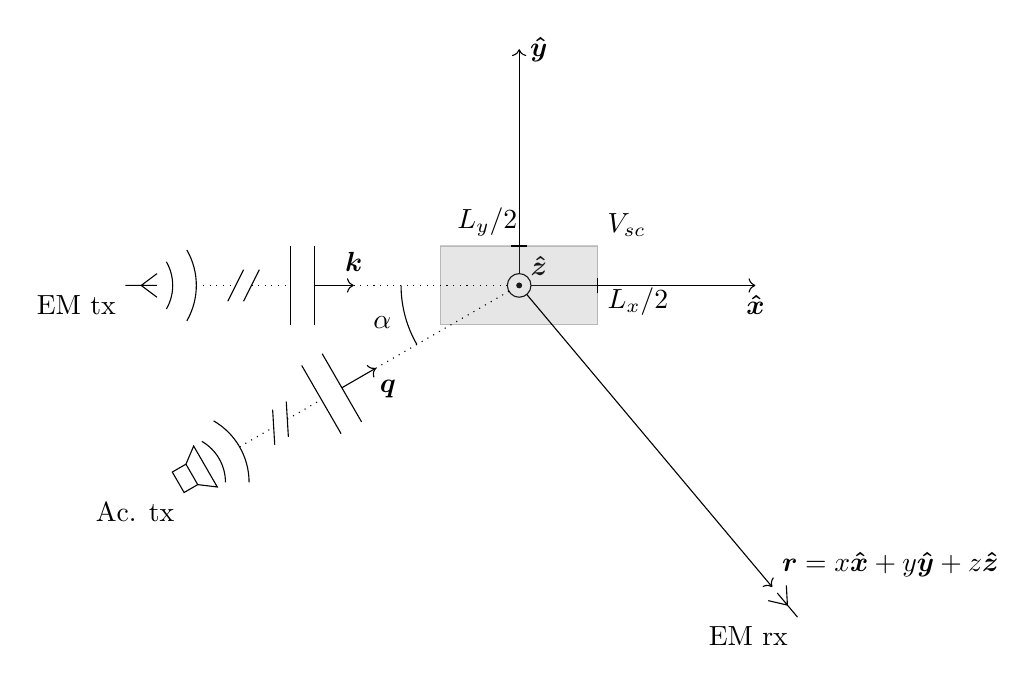
\begin{tikzpicture}
			% Draw coordinate axes
			\draw (0,0) circle(0.15);
			\filldraw[black] circle(0.03);
			\draw[->] (0.15,0) -- (3,0);
			\draw[->] (0,.150) -- (0,3);
			\draw (3,-0.25) node{$\bm{\hat{x}}$} (0.25,3) node{$\bm{\hat{y}}$} (0.25,0.25) node{$\bm{\hat{z}}$};
			
			% Draw scattering cube (or rectangle in this case)
			\draw[fill=gray,opacity=0.2] (-1,-0.5) rectangle(1,0.5);
			\draw (1,-0.1) -- (1,0.1) node[anchor= north west]{$L_{x}/2$} (-0.1,0.5) -- (0.1,0.5) node[anchor= south east]{$L_{y}/2$} (1,0.5) node[anchor=south west]{$V_\mrm{sc}$};
			
			% Draw EM tx and spherical waves
			\draw[shift = {(-5,0)}] (0,0) node[anchor=north east]{EM tx} -- (0.4,0) (0.2,0) -- (0.4,0.15)
			(0.2,0) -- (0.4,-0.15);
			\draw[shift = {(-5,0)}] ([shift={(-30:0.6)}] 0,0) arc(-30:30:0.6) ([shift={(-30:0.9)}] 0,0) arc(-30:30:0.9);
			
			% Draw EM "long distance" lines
			\draw[shift = {(-4.1,0)},dotted] (0,0) -- (0.5,0) (0.7,0) -- (1.2,0);
			\draw[shift = {(-4.1,0)}] (0.4,-0.2) -- (0.6,0.2) (0.6,-0.2) -- (0.8,0.2);
			
			% Draw EM plane waves
			\draw[shift = {(-2.9,0)}] (0,-0.5) -- (0,0.5) (0.3,-0.5) -- (0.3,0.5);
			\draw[shift = {(-2.6,0)}, ->] (0,0) -- (0.5,0);
			\draw[shift = {(-2.6,0)}] (0.5,0.3) node{$\bm{k}$};
			\draw[dotted] (-0.15,0) -- (-2.1,0);
			
			% Draw Ac. tx and spherical waves
			\draw[shift = {(210:5)}, rotate = 30] (0,-0.15) node[anchor=north east]{Ac. tx} rectangle (0.2,0.15) -- (0.4,0.3) -- (0.4,-0.3) -- (0.2,-0.15);
			\draw[shift = {(210:5)}, rotate = 30] ([shift={(-30:0.6)}] 0,0) arc(-30:30:0.6) ([shift={(-30:0.9)}] 0,0) arc(-30:30:0.9);
			
			% Draw Ac. "long distance" lines
			\draw[shift = {(210:4.1)}, rotate = 30,dotted] (0,0) -- (0.5,0) (0.7,0) -- (1.2,0);
			\draw[shift = {(210:4.1)}, rotate = 30] (0.4,-0.2) -- (0.6,0.2) (0.6,-0.2) -- (0.8,0.2);
			
			% Draw Ac. plane waves
			\draw[shift = {(210:2.9)}, rotate = 30] (0,-0.5) -- (0,0.5) (0.3,-0.5) -- (0.3,0.5);
			\draw[shift = {(210:2.6)}, rotate = 30, ->] (0,0) -- (0.5,0);
			\draw[shift = {(210:2.6)}, rotate = 30] (0.5,-0.3) node{$\bm{q}$};
			\draw[rotate = 30, dotted] (-0.15,0) -- (-2.1,0);
			
			% Draw angle alpha
			\draw ([shift={(180:1.5)}] 0,0) arc(180:210:1.5) (195:1.8) node{$\alpha$};
			
			% Draw line towards receiver
			\draw[->] (310:0.15) -- (310:5) node[anchor=south west]{$\bm{r} = x\bm{\hat{x}} + y\bm{\hat{y}} + z\bm{\hat{z}}$};
			
			% Draw EM rx
			\draw[shift = {(310:5.5)}, rotate = 130] (0,0) node[anchor=north east]{EM rx} -- (0.4,0) (0.2,0) -- (0.4,0.15) (0.2,0) -- (0.4,-0.15);
		\end{tikzpicture}
		}
		\caption{\label{fig:radareq-geom} Geometry for the scattering problem.}
	\end{figure}
	The $xy$-plane is defined as the plane formed by the acoustic and electromagnetic wavevectors (they are assumed to be non-parallel). The scattering volume is centered in the origin of the coordinate system, and both the acoustic and electromagnetic waves are approximated as plane waves close to the origin. Thus, the electromagnetic and dielectric perturbation fields near the origin are defined as
	\begin{align}
		\bm{E}_i (\bm{r}',t) &= \bm{E}_i (\bm{r}') = \bm{E}_{i0} e^{i\bm{k}\cdot\bm{r}'} \label{eq:app-radar-planeE} \\
		\varepsilon_1 (\bm{r}',t) &= -\mathfrak{p} \varepsilon_r^2 s_p \cos(\bm{q} \cdot \bm{r}' - \Omega t) \label{eq:app-radar-planeEps}
	\end{align}
	Here, $\bm{E}_{i0}$ is the complex field amplitude at the origin ($-i\omega t$ time-dependence separated) and $\bm{k}$ is the electromagnetic wavevector. A scalar photoelastic relation has been assumed, where $\mathfrak{p}$ is the photoelastic constant, $s_p$ is the acoustic strain amplitude at the origin, $\bm{q}$ is the acoustic wavevector and $\Omega$ the acoustic frequency.
	
	For simplicity, the electromagnetic polarization is assumed to be in z, $\bm{E}_{i0} \parallel \bm{\hat{z}}$. This is also in part done to avoid polarization changes in the scattered field \cite{Korpel1988}. Due to this $\nabla(\bm{E}_i \cdot \nabla \varepsilon_1) = \bm{0}$ which simplifies the scattering integral to
	\begin{equation*}
		\bm{E}_{sc}(\bm{r},t) = \frac{k^2}{4\pi\varepsilon_r} \int_{V_{sc}} \frac{e^{ik |\bm{r}-\bm{r'}| }}{ |\bm{r}-\bm{r'}|} \bm{E}_i (\bm{r'},t) \varepsilon_1 (\bm{r'},t) \mathrm{d}v'
	\end{equation*}
	Insertion of equation \eqref{eq:app-radar-planeE} and \eqref{eq:app-radar-planeEps} gives
	\begin{equation*}
		\bm{E}_{sc}(\bm{r},t) = -\frac{k^2}{4\pi\varepsilon_r} \int_{V_{sc}} \frac{e^{ik |\bm{r}-\bm{r'}| }}{ |\bm{r}-\bm{r'}|} \bm{E}_{i0} e^{i\bm{k} \cdot \bm{r}'} \mathfrak{p} \varepsilon_r^2 s_p \cos(\bm{q} \cdot \bm{r}' - \Omega t) \mathrm{d}v'
	\end{equation*}
	Assuming far-field gives an approximation for the Green-function as \cite{Kristensson2008}
	\begin{equation*}
		\frac{e^{ik |\bm{r}-\bm{r'}| }}{ |\bm{r}-\bm{r'}|} \approx \frac{e^{ikr}}{r} e^{-ik \bm{\hat{r}} \cdot \bm{r}'}
	\end{equation*}
	where $r = |\bm{r}|$ and $\bm{\hat{r}} = \bm{r}/r$. The scattering integral is now written as
	\begin{equation*}
		\bm{E}_{sc}(\bm{r},t) = -\frac{\varepsilon_rk^2 e^{ikr}}{4\pi r} \bm{E}_{i0} \mathfrak{p} s_p \int_{V_{sc}} e^{ik ( \bm{\hat{k}} - \bm{\hat{r}} ) \cdot \bm{r}'} \cos(\bm{q} \cdot \bm{r}' - \Omega t) \mathrm{d}v'
	\end{equation*}
	The cosine is now written as complex exponentials giving
	\begin{equation*}
	\begin{split}
			\bm{E}_{sc}(\bm{r},t) =& -\frac{\varepsilon_rk^2 e^{ikr}}{8\pi r} \bm{E}_{i0} \mathfrak{p} s_p \\
			&\cdot \left( e^{-i\Omega t} \int_{V_{sc}} e^{i( k(\bm{\hat{k}} - \bm{\hat{r}}) + \bm{q} ) \cdot \bm{r}'} \mathrm{d}v + e^{i\Omega t} \int_{V_{sc}} e^{i( k(\bm{\hat{k}} - \bm{\hat{r}}) - \bm{q} ) \cdot \bm{r}'} \mathrm{d}v' \right)
	\end{split}
	\end{equation*}
	The two integrals are of the same form, $\int e^{i\bm{A} \cdot \bm{r}'} \mathrm{d}v'$, where $\bm{A}$ is independent of $\bm{r}'$. This is solved in general below for the cuboid volume defined by $-L_m/2 \leq m \leq L_m/2$, $m = x,y,z$.
	\begin{equation*}
	\begin{split}
		\int_{V_{sc}} e^{i\bm{A} \cdot \bm{r}'} \mathrm{d}v' &=
		\int_{V_{sc}} e^{i\bm{A} \cdot \bm{\hat{x}} x'} e^{i\bm{A} \cdot \bm{\hat{y}} y'} e^{i\bm{A} \cdot \bm{\hat{z}} z'} \mathrm{d}v' \\
		&= \prod_{m = x,y,z} \frac{1}{i \bm{A} \cdot \bm{\hat{m}}} \left( e^{i\bm{A} \cdot \bm{\hat{m}} L_m/2} - e^{-i\bm{A} \cdot \bm{\hat{m}} L_m/2} \right) \\
		&= \prod_{m = x,y,z} \frac{2}{\bm{A} \cdot \bm{\hat{m}}} \sin \left(\bm{A} \cdot \bm{\hat{m}} \frac{L_m}{2} \right) 
		= \prod_{m = x,y,z} L_m \text{sinc} \left( \frac{\bm{A} \cdot \bm{\hat{m}} L_m}{2\pi} \right)
	\end{split}
	\end{equation*}
	where sinc$(x) = \sin(\pi x)/(\pi x)$. To apply this result to $\bm{A} = k(\bm{\hat{k}} - \bm{\hat{r}}) \pm \bm{q}$ this is first simplified using the geometry defined earlier.
	\begin{equation*}
		k(\bm{\hat{k}} - \bm{\hat{r}}) \pm \bm{q} = k\bm{\hat{x}} - k(\bm{\hat{x}} x + \bm{\hat{y}} y + \bm{\hat{z}} z)/r \pm q(\bm{\hat{x}} \cos{\alpha} + \bm{\hat{y}} \sin{\alpha})
	\end{equation*}
	where r is not written out fully. $\bm{A} \cdot \bm{\hat{m}}$ are now calculated for the three coordinate axes as
	\begin{equation} 
	\begin{split}
		\bm{A} \cdot \bm{\hat{x}} &= k - kx/r \pm q\cos{\alpha} = k - k\sin{\theta}\cos{\phi} \pm q\cos{\alpha} \\
		\bm{A} \cdot \bm{\hat{y}} &= - ky/r \pm q\sin{\alpha} = - k\sin{\theta}\sin{\phi} \pm q\sin{\alpha} \\
		\bm{A} \cdot \bm{\hat{z}} &= -kz/r = -k\cos{\theta}
	\end{split}
	\label{eq:radar-Aproj}
	\end{equation}
	where a conversion to spherical coordinates was made. Insertion into the integral solution gives:
	\begin{equation}
		\begin{split} 
			\int_{V_{sc}} &e^{i(	k(\bm{\hat{k}} - \bm{\hat{r}}) \pm \bm{q}) \cdot \bm{r}'} \mathrm{d}v' \\
			=& L_x \text{sinc} \left( \frac{L_x}{2\pi} ( k - k\sin{\theta}\cos{\phi} \pm q\cos{\alpha} ) \right) \\
			&\cdot L_y \text{sinc} \left( \frac{L_y}{2\pi} ( - k\sin{\theta}\sin{\phi} \pm q\sin{\alpha} ) \right)
			\cdot L_z \text{sinc} \left( -\frac{L_z}{2\pi} k\cos{\theta} \right) \\
			=& L_x L_y L_z \Phi^\pm (\theta,\phi)
		\end{split}
		\label{eq:radar-intsol}
	\end{equation}
	
	
	where all angular dependence has been gathered in the function $\Phi^\pm (\theta,\phi)$. This result is now inserted into the scattered field, giving
	\begin{equation*}
	\begin{split}
		\bm{E}_{sc}(\bm{r},t) &= -\bm{E}_{i0} \frac{\varepsilon_rk^2 e^{ikr}}{8\pi r} \mathfrak{p} s_p L_x L_y L_z \left( e^{-i\Omega t} \Phi^+ (\theta,\phi)  + e^{i\Omega t} \Phi^- (\theta,\phi) \right) \\
		&= -\bm{E}_{i0} E_A(\bm{r},t)
	\end{split}
	\end{equation*}
	
	By inspecting $E_A(\bm{r},t)$ it is clear that two frequency-shifted components arise. Since the implied time-dependence is $e^{-i\omega t}$, the factors $e^{\mp i\Omega t}$ give a frequency shift of $\pm \Omega$. The scattered field is written using two distinct components as
	\begin{equation*}
		\bm{E}_{sc} (\bm{r},t) = -\bm{E}_{i0} \left( E_A^+ (\bm{r},t) + E_A^- (\bm{r},t) \right)
	\end{equation*}
	where
	\begin{equation*}
		E_A^\pm (\bm{r},t) = \frac{\varepsilon_rk^2 e^{ikr}}{8\pi r} \mathfrak{p} s_p L_x L_y L_z e^{\mp i\Omega t} \Phi^\pm (\theta,\phi)
	\end{equation*}
	
	\subsection{Solution in terms of power}
	This treatment has primarily been focused around the electric field. To obtain a more practical expression, this is now transformed into power. The time average on the short time-scale ($\omega$, not $\Omega$) of the Poynting vector is \cite{Kristensson2008}
	\begin{equation*}
		\left< \bm{S}_{sc} \right> = \frac{1}{2} \mathrm{Re}\left\{ \bm{E}_{sc} \times \bm{H}_{sc}^* \right\}
	\end{equation*}
	where the E- and H-fields are complex with long time-scale time dependence. The magnetic field $\bm{H}_{sc}$ is given by \cite{Kristensson2008}
	\begin{equation*}
		\bm{H}_{sc} \approx \frac{1}{ik \eta_0 \eta} \nabla \times \bm{E}_{sc}
	\end{equation*}
	where $\eta_0$ is the wave impedance of free space and $\eta_0 \eta$ the wave impedance in the material. An approximation has been made for $k$, where this is assumed to have the same value as before scattering. Since there is a frequency shift this is known to not be the case, but given a small acoustic frequency compared to the electromagnetic frequency, the error is small. The curl of $\bm{E}_{sc}$ is now written as
	\begin{equation*}
		\nabla \times \bm{E}_{sc} = -\nabla \times (\bm{E}_{i0} E_A (\bm{r},t)) = -\nabla E_A (\bm{r},t) \times \bm{E}_{i0}
	\end{equation*}
	In spherical coordinates the gradient is written \addref
	\begin{equation*}
		\nabla E_A = \frac{\partial E_A}{\partial r} \bm{\hat{r}} + \frac{1}{r} \frac{\partial E_A}{\partial \theta} \bm{\hat{\theta}} + \frac{1}{r\sin{\theta}} \frac{\partial E_A}{\partial \phi} \bm{\hat{\phi}}
	\end{equation*}
	$E_A$ contains a factor $1/r$, so the two last terms in the gradient will be $\sim 1/r^2$ and are neglected. The gradient is now written as
	\begin{equation*}
	\begin{split}
		\nabla E_A &\approx \frac{\partial E_A}{\partial r} \bm{\hat{r}} \\
		&= \left( \frac{ike^{ikr}}{r} - \frac{e^{ikr}}{r^2} \right) \frac{\varepsilon_r k^2}{8\pi} \mathfrak{p} S_0 L_x L_y L_z \left( e^{- i\Omega t} \Phi^+ (\theta,\phi) + e^{ i\Omega t} \Phi^- (\theta,\phi) \right) \bm{\hat{r}} \\
		&\approx ikE_A \bm{\hat{r}}
	\end{split}
	\end{equation*}
	where the $1/r^2$ term was neglected. These results are inserted into the expression for the magnetic field, giving
	\begin{equation*}
		\bm{H}_{sc} = \frac{1}{ik \eta_0 \eta} (-ikE_A \bm{\hat{r}} \times \bm{E}_{i0}) = \frac{E_A}{ \eta_0 \eta} \bm{\hat{r}} \times \bm{E}_{i0}
	\end{equation*}
	Now, the cross product with the electric field is calculated as
	\begin{equation*}
		\bm{E}_{sc} \times \bm{H}_{sc}^* = E_A \bm{E}_{i0} \times \left( \frac{E_A}{ \eta_0 \eta} \bm{\hat{r}} \times \bm{E}_{i0} \right)^* = \frac{|E_A|^2}{\eta_0 \eta} \left( \bm{\hat{r}} (\bm{E}_{i0} \cdot \bm{E}_{i0}^*) - \bm{E}_{i0}^* (\bm{E}_{i0} \cdot \bm{\hat{r}}) \right)
	\end{equation*}
	In the far-field $\bm{E}_{sc} \cdot \bm{\hat{r}} = 0$ \addref and since $\bm{E}_{sc} \parallel \bm{E}_{i0}$ the cross product is simplified to
	\begin{equation*}
		\bm{E}_{sc} \times \bm{H}_{sc}^* = \frac{\bm{\hat{r}}}{\eta_0 \eta} |\bm{E}_{i0}|^2 |E_A (\bm{r},t)|^2
	\end{equation*}
	The time-averaged Poynting vector is now calculated as
	\begin{equation*}
		\left< \bm{S}_{sc} \right> = \frac{1}{2}\mathrm{Re}\left\{ \bm{E}_{sc} \times \bm{H}_{sc}^* \right\} = \frac{\bm{\hat{r}}}{2\eta_0 \eta} |\bm{E}_{i0}|^2 |E_A (\bm{r},t)|^2
	\end{equation*}
	If the two frequency components are now considered individually,
	\begin{equation*}
		|E_A^\pm (\bm{r},t)|^2 =\frac{\varepsilon_r^2 k^4}{64 \pi^2 r^2} \mathfrak{p}^2 S_0^2 L_x^2 L_y^2 L_z^2 \Phi^\pm (\theta,\phi)^2
	\end{equation*}
	
	To find an expression for $|\bm{E}_{i0}|^2$, the field from the transmitter antenna is written as (adapted from \cite{Orfanidis2016})
	\begin{equation*}
		\bm{E}_T (\bm{r}) = ik\eta_0\eta \frac{e^{ikr}}{4\pi r} \bm{F}_\perp (\bm{\hat{r}})
	\end{equation*}
	where $\bm{F}_\perp$ is the far-field amplitude. Now the coordinate system is not the same as earlier in the derivation! Here it is a spherical coordinate system with origin at the transmitting antenna. This corresponds to a translation in $-\bm{\hat{x}}$ of the original coordinate system. Let $R_T$ be the distance between the two coordinate systems, or equivalently the distance from the transmitter to the scattering center. The direction to the scattering center in this new system is denoted $\bm{\hat{r}}_{sc} = \bm{r}_{sc}/R_T$. Assuming that the orientations of the transmitter and scattering coordinate systems are the same, $|\bm{E}_{i0}|^2$ can be written in the transmitter system as \cite{Orfanidis2016}
	\begin{equation*}
		|\bm{E}_{i0}|^2 = |\bm{E}_T(\bm{r}_{sc})|^2 = \left| ik\eta_0\eta \frac{e^{ikR_T}}{4\pi R_T} \bm{F}_\perp (\bm{\hat{r}}_{sc}) \right|^2 = \frac{k^2 \eta_0^2 \eta^2}{16 \pi^2 R_T^2} |\bm{F}_\perp (\bm{\hat{r}}_{sc})|^2 = 2\eta_0 \eta \mathcal{P}(\bm{\hat{r}}_{sc})
	\end{equation*}
	If the maximum gain $G_T$ of the antenna is in the direction $\hat{r}_{sc}$, it holds that \cite{Orfanidis2016}
	\begin{equation*}
		\mathcal{P}(\bm{\hat{r}}_{sc}) = \frac{P_T G_T}{4\pi R_T^2}
	\end{equation*}
	where $P_T$ is the power accepted by the antenna. This is used to write
	\begin{equation*}
		|\bm{E}_{i0}|^2 = 2\eta_0 \eta \frac{P_T G_T}{4\pi R_T^2}
	\end{equation*}
	Now this is inserted into the time-average of the power density
	\begin{equation*}
		\left< \bm{S}_{sc} \right>^\pm = \bm{\hat{r}} \frac{P_T G_T}{4\pi R_T^2} \frac{\varepsilon_r^2 k^4}{64 \pi^2 r^2} \mathfrak{p}^2 S_0^2 L_x^2 L_y^2 L_z^2 \Phi^\pm (\theta,\phi)^2
	\end{equation*}
	
	Now the effects of the receiving antenna are considered. It is assumed that this antenna is optimally directed towards the scattering center. The received power is then
	\begin{equation*}
		P_R^\pm = \left| \left< \bm{S}_{sc} \right>^\pm \right| A_e
	\end{equation*}
	where $A_e$ is the effective area of the antenna, which can be rewritten as
	\begin{equation*}
		A_e = \frac{\lambda_R^2 G_R}{4\pi}
	\end{equation*}
	where $G_R$ is the gain of the receiving antenna. $\lambda_R$ should be the wavelength at the antenna here, which is not necessarily the same as in the material. Combining this with earlier results gives a received power of
	\begin{equation*}
		P_R^\pm = \frac{\lambda_R^2 G_R}{4\pi} \frac{P_T G_T}{4\pi R_T^2} \frac{\varepsilon_r^2 k^4}{64 \pi^2 R_R^2} \mathfrak{p}^2 S_0^2 L_x^2 L_y^2 L_z^2 \Phi^\pm (\theta,\phi)^2
	\end{equation*}
	where $R_R$ is the distance between the scattering center and the receiver, and the receiver is located in the direction $(\theta,\phi)$ as seen from the scattering center. For a more traditional bistatic radar equation this can be written as
	\begin{equation*}
		P_R^\pm = \frac{P_T G_T G_R \lambda_R^2 \sigma^\pm (\theta,\phi)}{(4\pi)^3 R_T^2 R_R^2}
	\end{equation*}
	with the radar cross-section given by
	\begin{equation*}
		\sigma^\pm (\theta, \phi) = \frac{\varepsilon_r^2 k^4}{16\pi} \mathfrak{p}^2 S_0^2 L_x^2 L_y^2 L_z^2 \Phi^\pm (\theta,\phi)^2
	\end{equation*}
	
	\subsection{Signal-to-noise ratio and coherent integration}
	A more practical measurement than received power is signal-to-noise ratio (SNR). For this, the average noise power is described as \cite{Young2004}
	\begin{equation*}
		P_n = k_B TB
	\end{equation*}
	where $k_B$ is Boltzmann's constant, $T$ is the temperature and $B$ is the utilized receiver bandwidth. The noise power picked up by the antenna is calculated using the standard temperature $T_0 = 290$ K. The SNR directly at the antenna can thus be written as
	\begin{equation*}
		\mathit{SNR}^\pm_{ant} \frac{P_T G_T G_R \lambda_R^2 \sigma^\pm (\theta,\phi)}{(4\pi)^3 R_T^2 R_R^2 k_B T_0 B}
	\end{equation*}
	After the antenna is the RF front-end which usually contains a bandpass filter, low-noise amplifier (LNA), and mixer. Here the received signal is amplified so that it can be further processed. The amplification affects both the signal and noise, but the electronic components add more noise which causes the SNR to deteriorate. To quantify this, the concept of noise ratio and noise figure is used. The noise ratio is defined as \cite{Young2004}
	\begin{equation*}
		F = \frac{\mathit{SNR}_i}{\mathit{SNR}_o}
	\end{equation*}
	where the SNR's are in linear units, $i$ denotes input and $o$ denotes output. It is more common to use noise figure, which is simply the noise ratio expressed in dB units, $\mathit{NF} = 10\log_{10}(F)$. After the RF front-end the signal is often strong enough to not be affected by further noise, so it is usually sufficient to use a noise ratio/figure for that part of the receiver. The SNR after the receiver can now be written using the noise ratio as
	\begin{equation*}
		\mathit{SNR}^\pm = \frac{P_T G_T G_R \lambda_R^2 \sigma^\pm (\theta,\phi)}{(4\pi)^3 R_T^2 R_R^2 k_B T_0 B \cdot F}
	\end{equation*}
	One more effect is added to this, and that is signal integration in the signal processing following the receiver. Noise can often be modeled as a random process, and if multiple samples are added together the noise can be averaged out. If coherent demodulation is used, $N$ samples added together will cause the SNR to improve by a factor $N$ \cite{Richards2012}. The SNR can then be written as
	\begin{equation*}
		\mathit{SNR}^\pm_N = \frac{P_T G_T G_R \lambda_R^2 \sigma^\pm (\theta,\phi)}{(4\pi)^3 R_T^2 R_R^2 k_B T_0 B F} N
	\end{equation*}
	
	\section{Refined interaction region} \label{sec:app-derivations-refined}
	The derivation in \ref{sec:app-derivations-radar} is based on plane waves and a very simple geometry. A problem with the geometry used is that there is no easy way to obtain the parameters $L_x$, $L_y$ and $L_z$ from common parameters of the acoustic and electromagnetic beams. To address this, a slightly different interaction geometry based on beams is introduced as shown in figure \ref{fig:parallelogram}. Here the beam diameters $d_e$ and $d_a$ have been introduced for the electromagnetic and acoustic plane waves. For simplicity, it is assumed that the beam edges are infinitely sharp, i.e. inside the wave behaves as a plane wave and outside it is zero. This way the previous derivation can be used with the exception of the interaction region.
	\begin{figure}[h]
		\centering
		\resizebox{\textwidth}{!}{
			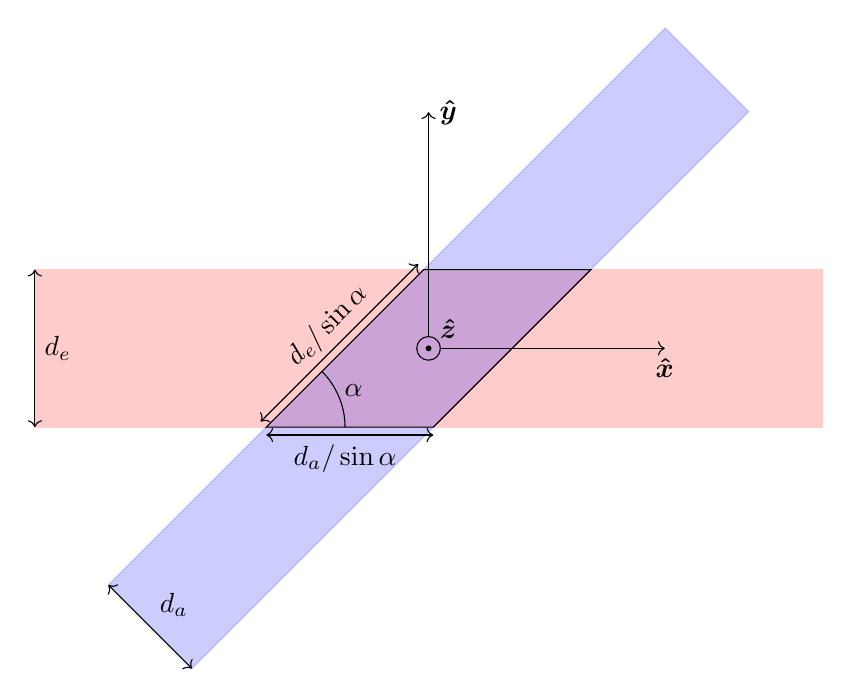
\begin{tikzpicture}
	
	
	% Draw EM beam
	\filldraw[red,opacity=0.2] (-5,-1) rectangle(5,1);
	\draw[<->] (-5,-1) -- (-5,1);
	\draw (-5,0) node[anchor=west]{$d_e$};
	
	% Draw Ac beam
	\filldraw[blue,rotate=45,opacity=0.2] (-5,-0.75) rectangle(5,0.75);
	\draw[<->,rotate=45] (-5,-0.75) -- (-5,0.75);
	\draw[rotate=45] (-5,0) node[anchor=south west]{$d_a$};
	
	% Draw parallelogram
	\draw (-2.061,-1) -- (-0.061,1) -- (2.061,1) -- (0.061,-1) -- cycle;
	\draw[<->] (-2.061,-1.1) -- (0.061, -1.1);
	\draw (-1.061, -1.4) node{$d_a/\sin{\alpha}$};
	\draw[<->, shift={(135:0.1)}] (-2.061,-1) -- (-0.061,1);
	\draw[shift={(135:0.4)}] (-1,0) node[anchor=center,rotate=45] {$d_e/\sin{\alpha}$};
	
	% Draw angle alpha
	\draw ([shift={(-1.061,-1)}] 0,0) arc(0:45:1) ([shift={(22.5:1.2)}] -2.061,-1) node{$\alpha$};
	
	% Draw coordinate axes
	\draw (0,0) circle(0.15);
	\filldraw[black] circle(0.03);
	\draw[->] (0.15,0) -- (3,0);
	\draw[->] (0,.150) -- (0,3);
	\draw (3,-0.25) node{$\bm{\hat{x}}$} (0.25,3) node{$\bm{\hat{y}}$} (0.25,0.25) node{$\bm{\hat{z}}$};
	
\end{tikzpicture}
		}
		\caption{\label{fig:parallelogram} Parallelogram interaction region}
	\end{figure}
	Since plane waves are still used the model is not based on real beams. However, for real beams it is still easy to obtain widths at the overlap area and then the interaction region should be fairly close using this model.
	
	The integration limits corresponding to this parallelogram can be written as
	\begin{align*}
		x_0 - x_1 &< x < x_0 + x_1 \\
		-d_e/2 &< y < d_e/2 \\
		-L_z/2 &< z < L_z/2
	\end{align*}
	where
	\begin{align*}
		x_0 &= \frac{y}{\tan{\alpha}} \\
		x_1 &= \frac{d_a}{2\sin{\alpha}}
	\end{align*}
	The solution to the integral for a general function on the form $e^{i\bm{A} \cdot \bm{r}}$ is now written as
	\begin{equation*}
	\begin{split}
			I &= \int_{V_{sc}} e^{i\bm{A} \cdot \bm{r}'} \mathrm{d}v' \\
			&= \int_{-L_z/2}^{L_z/2} e^{i\bm{A} \cdot \bm{\hat{z}} z'} \mathrm{d}z'
			\int_{-d_e/2}^{d_e/2} \left( e^{i\bm{A} \cdot \bm{\hat{y}} y'}
			\int_{x_0-x_1}^{x_0+x_1} e^{i\bm{A} \cdot \bm{\hat{x}} x'} \mathrm{d}x' \right) \mathrm{d}y' \\
			&= \int_{-L_z/2}^{L_z/2} e^{i\bm{A} \cdot \bm{\hat{z}} z'} \mathrm{d}z' \cdot I_2
	\end{split}
	\end{equation*}
	using the solution from \ref{sec:app-derivations-radar} \todoint{Maybe make better references?} this integral can be written as
	\begin{equation*}
		I = L_z \text{sinc}\left( \frac{\bm{A} \cdot \bm{\hat{z}} L_z}{2\pi} \right) \cdot I_2
	\end{equation*}
	The integral $I_2$ can be solved as
	\begin{equation*}
	\begin{split}
		I_2 &= \int_{-d_e/2}^{d_e/2} e^{i\bm{A} \cdot \bm{\hat{y}} y'}
		\cdot \frac{1}{i\bm{A} \cdot \bm{\hat{x}}}
		\left( e^{i\bm{A} \cdot \bm{\hat{x}} (x_0+x_1)} - e^{i\bm{A} \cdot \bm{\hat{x}} (x_0-x_1)}\right) \mathrm{d}y' \\
		&=\int_{-d_e/2}^{d_e/2} e^{i\bm{A} \cdot \bm{\hat{y}} y'}
		\cdot e^{i\bm{A} \cdot \bm{\hat{x}} x_0} \frac{2}{\bm{A} \cdot \bm{\hat{x}}} \sin(\bm{A} \cdot \bm{\hat{x}} x_1) \mathrm{d}y' \\
		&=\int_{-d_e/2}^{d_e/2} e^{i\bm{A} \cdot (\bm{\hat{y}} y'+ \bm{\hat{x}} x_0)}
		\cdot 2x_1 \text{sinc}\left( \frac{\bm{A} \cdot \bm{\hat{x}} x_1}{\pi} \right) \mathrm{d}y' \\
		&= \frac{d_a}{\sin{\alpha}} \text{sinc}\left( \frac{\bm{A} \cdot \bm{\hat{x}} d_a}{2\pi \sin{\alpha}} \right) \int_{-d_e/2}^{d_e/2} e^{i\bm{A} \cdot (\bm{\hat{y}} + \bm{\hat{x}}/\tan{\alpha}) y'} \mathrm{d}y' \\
		&= \frac{d_a}{\sin{\alpha}} \text{sinc}\left( \frac{\bm{A} \cdot \bm{\hat{x}} d_a}{2\pi \sin{\alpha}} \right) \cdot I_3
	\end{split}
	\end{equation*}
	The integral $I_3$ can be solved analogously to the solution from \ref{sec:app-derivations-radar} as
	\begin{equation*}
		I_3 = d_e \text{sinc}\left( \frac{\bm{A} \cdot (\bm{\hat{y}} + \bm{\hat{x}}/\tan{\alpha}) d_e}{2\pi} \right)
	\end{equation*}
	Now the complete solution to $I$ is written as
	\begin{equation*}
	\begin{split}
		I =& \frac{d_a}{\sin{\alpha}} \text{sinc}\left( \frac{\bm{A} \cdot \bm{\hat{x}} d_a}{2\pi \sin{\alpha}} \right) \cdot d_e \text{sinc}\left( \frac{\bm{A} \cdot (\bm{\hat{y}} + \bm{\hat{x}}/\tan{\alpha}) d_e}{2\pi} \right) \\
		&\cdot L_z \text{sinc}\left( \frac{\bm{A} \cdot \bm{\hat{z}} L_z}{2\pi} \right)
	\end{split}
	\end{equation*}
	If the specific function of interest to the scattering problem is inserted, and spherical coordinates are used as in equation \eqref{eq:radar-Aproj} the solution is
	\begin{equation*}
	\begin{split}
		\int_{V_{sc}} &e^{i(	k(\bm{\hat{k}} - \bm{\hat{r}}) \pm \bm{q}) \cdot \bm{r}'} \mathrm{d}v' \\
		&= \frac{d_a d_e L_z}{\sin{\alpha}} \text{sinc}\left( \frac{d_a}{2\pi \sin{\alpha}}(k - k\sin{\theta}\cos{\phi} \pm q\cos{\alpha}) \right) \\
		&\cdot \text{sinc}\left( \frac{d_e}{2\pi \tan{\alpha}}
		(k - k\sin{\theta}(\cos{\phi} + \sin{\phi}\tan{\alpha}) \pm q(\cos{\alpha} + \sin{\alpha}\tan{\alpha})) \right) \\
		&\cdot \text{sinc}\left( -\frac{L_z}{2\pi} k\cos{\theta} \right) \\
		&= \frac{d_a d_e L_z}{\sin{\alpha}} \Phi_p^{\pm}(\theta, \phi)
	\end{split}
	\end{equation*}
	where the function $\Phi_p^{\pm}(\theta, \phi)$ was introduced similarly to $\Phi^{\pm}(\theta, \phi)$ in equation \eqref{eq:radar-intsol}. In contrast to the derivation in \ref{sec:app-derivations-radar}, $\Phi_p^{\pm}(\theta, \phi)$ does not contain all angular dependence since there is still a factor $1/\sin{\alpha}$ not included. This is due to that factor being directly related to the interaction volume. If the area of the parallelogram is calculated and multiplied by the width in $z$, the result is
	\begin{equation*}
		\frac{d_a d_e L_z}{\sin{\alpha}}
	\end{equation*}
	This means that the solution of the integral is the interaction volume multiplied by $\Phi_p^{\pm}(\theta, \phi)$. This is the same result as in equation \eqref{eq:radar-intsol}.
	
	For the major results of the derivations in section \ref{sec:app-derivations-radar}, the interaction region is easily changed from cuboid to beam-based. The geometry only matters in the calculation of the integral, so the only necessary changes are from there. This means that the interaction volume needs to be changed from $L_x L_y L_z$ to $d_a d_e L_z/\sin{\alpha}$ and the function $\Phi^\pm$ changed to $\Phi_p^\pm$. The same expressions as before for electric fields, received power, SNR, etc. can be used if these changes are made.
	
	\section{Geometry for maximum scattering \label{sec:app-derivations-bragg}}
	Let us begin with the $\Phi$ angular dependence function:
	\begin{equation*}
	\begin{split}
		\Phi^\pm(\theta,\phi) =& \text{sinc} \left( \frac{L_x}{2\pi} \left( k - k\sin{\theta}\cos{\phi} \pm q\cos{\alpha} \right) \right) \\
		\cdot& \text{sinc} \left( \frac{L_y}{2\pi} \left( -k\sin{\theta}\sin{\phi} \pm q\sin{\alpha} \right) \right) \\
		\cdot& \text{sinc} \left( -\frac{L_z}{2\pi} k\cos{\theta} \right)
	\end{split}
	\end{equation*}
	The maximum of this function mush be where all sinc-functions are maximum. For a sinc the maximum is given when the argument is equal to 0, which simplifies the process. Firstly, consider the third sinc:
	\begin{equation*}
		\text{sinc} \left( -\frac{L_z}{2\pi} k\cos{\theta} \right)
	\end{equation*}
	The argument of this is obviously zero when $\cos{\theta} = 0$, which for $0 \leq \theta \leq \pi$ is when $\theta = \pi/2$. This fixes the maximum to the plane formed by the incident electromagnetic and acoustic wavevectors. What it means is that the scattering occurs primarily in one single interaction plane, which simplifies analysis. Now the arguments of the two other sinc functions are set to zero with the value for $\theta$ being set to $\pi/2$:
	\begin{align}
		k - k\cos{\phi} \pm q\cos{\alpha} &= 0 \label{eq:app-bragg-sinc1} \\
		-k\sin{\phi} \pm q\sin{\alpha} &= 0 \label{eq:app-bragg-sinc2}
	\end{align}
	
	\subsection{Condition for $\alpha$}
	The system \eqref{eq:app-bragg-sinc1},\eqref{eq:app-bragg-sinc2} is now used to find the angle between wave vectors giving a maximum. To avoid confusion, the positive and negative versions of the system are considered separately.
	
	\subsubsection{(+) case}
	Begin with equation \eqref{eq:app-bragg-sinc1}:
	\begin{equation*}
		\cos{\alpha} = \frac{k}{q}\left( \cos{\phi} - 1 \right) = \frac{k}{q}\left( \pm \sqrt{1-\sin^2{\phi}} - 1 \right)
	\end{equation*}
	Now equation \eqref{eq:app-bragg-sinc2} is inserted in the above as
	\begin{equation*}
		\cos{\alpha} = \frac{k}{q}\left( \pm \sqrt{1-\frac{q^2}{k^2}\sin^2{\alpha}} - 1 \right)
	\end{equation*}
	This is rewritten as
	\begin{equation*}
		\pm \sqrt{k^2-q^2\sin^2{\alpha}} = q\cos{\alpha} + k
	\end{equation*}
	And squared
	\begin{equation*}
		k^2 - q^2\sin^2{\alpha} = q^2\cos^2{\alpha} + 2kq\cos{\alpha} + k^2
	\end{equation*}
	After some simplification, the following equation is obtained:
	\begin{equation}
		\cos{\alpha} = -\frac{q}{2k} \label{eq:app-bragg-cos+}
	\end{equation}
	Since $q$ and $k$ are non-negative it is clear that $\pi/2 \leq \alpha \leq \pi$.
	
	\subsubsection{(-) case}
	This case is the same as the (+) case, but with some sign changes. Begin with equation \eqref{eq:app-bragg-sinc1}:
	\begin{equation*}
		\cos{\alpha} = \frac{k}{q}\left( 1 - \cos{\phi} \right) = \frac{k}{q}\left( 1 \pm \sqrt{1-\sin^2{\phi}} \right)
	\end{equation*}
	Now equation \eqref{eq:app-bragg-sinc2} is inserted in the above as
	\begin{equation*}
		\cos{\alpha} = \frac{k}{q}\left( 1 \pm \sqrt{1-\frac{q^2}{k^2}\sin^2{\alpha}} \right)
	\end{equation*}
	This is rewritten as
	\begin{equation*}
		\pm \sqrt{k^2-q^2\sin^2{\alpha}} = q\cos{\alpha} - k
	\end{equation*}
	And squared
	\begin{equation*}
		k^2 - q^2\sin^2{\alpha} = q^2\cos^2{\alpha} - 2kq\cos{\alpha} + k^2
	\end{equation*}
	After some simplification, the following equation is obtained:
	\begin{equation}
		\cos{\alpha} = \frac{q}{2k} \label{eq:app-bragg-cos-}
	\end{equation}
	Since $q$ and $k$ are non-negative it is clear that $0 \leq \alpha \leq \pi/2$.

	\subsection{Condition for $\phi$}
	If either of equations \eqref{eq:app-bragg-cos+} or \eqref{eq:app-bragg-cos-} is inserted in the system \eqref{eq:app-bragg-sinc1}, \eqref{eq:app-bragg-sinc2} the following is obtained:
	\begin{align*}
		\cos{\phi} &= 1 - 2\cos^2{\alpha} = -\cos{2\alpha} \\
		\sin{\phi} &= -2\sin{\alpha}\cos{\alpha} = -\sin{2\alpha}
	\end{align*}
	These can be written as
	\begin{align*}
		\phi &=
		\begin{cases}
			\arccos(-\cos{2\alpha}) + 2\pi n &= \pi - 2\alpha + 2\pi n \\
			2\pi - \arccos(-\cos{2\alpha}) + 2\pi n &= \pi + 2\alpha + 2\pi n
		\end{cases} \\
		\phi &=
		\begin{cases}
			\arcsin(-\sin{2\alpha}) + 2\pi n &= -2\alpha + 2\pi n \\
			\pi - \arcsin(-\sin{2\alpha}) + 2\pi n &= \pi + 2\alpha + 2\pi n
		\end{cases}
	\end{align*}
	From these equations it is clear that $\phi = \pi + 2\alpha + 2\pi n$ is the only valid solution. If $\phi$ is constrained to the region $0 \leq \phi \leq 2\pi$ and the previously stated constraints on $\alpha$ are utilized, $\phi$ can be written as
	\begin{align*}
		\phi &= -\pi + 2\alpha \text{ (+ case)}\\
		\phi &= \pi + 2\alpha \text{ (- case)}
	\end{align*}
	
	\subsection{Summary}
	The equations for both the (+) and (-) case are very similar, and can be written in a simple way using $\pm$ signs. The conditions define the geometry which gives the maximum scattering through the angle $\alpha$ between EM and acoustic incident waves and the angles $\theta$ and $\phi$ for the receiver direction. They are summarized below:
	\begin{align}
		\theta &= \pi/2 \label{eq:app-bragg-theta}\\
		\cos{\alpha} = \mp \frac{q}{2k} &= \mp \frac{\lambda}{2\Lambda} \label{eq:app-bragg-alpha}\\
		\phi &= \mp \pi + 2\alpha \label{eq:app-bragg-phi}
		%\tan{\frac{\phi}{2}} = \pm \sqrt{\frac{q^2}{4k^2-q^2}} &= \pm \sqrt{\frac{\lambda^2}{4\Lambda^2-\lambda^2}} \label{eq:bragg-phi}
	\end{align}
	
	In acousto-optics the interaction occurs in a single plane, which is what \eqref{eq:app-bragg-theta} describes. There is also a Bragg condition defining the angle between an acoustic and optic wave which is required for maximum reflection. This is presented in \cite{Saleh2007} as
	\begin{equation*}
		\sin{\theta_B} = \frac{\lambda}{2\Lambda}
	\end{equation*}
	The relationship between the angles in acousto-optics and those used in this model are shown in figure \ref{fig:bragg-comparison} with $\phi_i = \phi_r = \theta_B$ \cite{Saleh2007}. From the figure it is clear that $\alpha = \pi/2 \pm \theta_B$. In this model \eqref{eq:app-bragg-alpha} is used to obtain the optimal angle between electromagnetic and acoustic waves, and the transformation between $\alpha$ and $\theta_B$ can be inserted as
	\begin{equation*}
		\cos{\alpha} = \cos(\pi/2 \pm \theta_B) = \mp \sin{\theta_B}
	\end{equation*}
	The RHS of \eqref{eq:app-bragg-alpha} is $\mp \lambda/2\Lambda$. This should be equal to the RHS above, which directly gives the Bragg condition.
	
	In acousto-optics it is assumed that the reflection angle equals the incidence angle. This is not directly stated here, but can be obtained by changing from the angles $\alpha$, $\phi$ to the incidence angle $\phi_i$ and reflection angle $\phi_r$ shown in figure \ref{fig:bragg-comparison}. It is clear from the figure that
	\begin{align*}
		\phi_i &= \pm(\alpha - \pi/2) \\
		\phi_r &=
		\begin{cases}
			\phi - \phi_i &\text{ (+ case)} \\
			2\pi - \phi - \phi_i &\text{ (- case)}
		\end{cases}
	\end{align*}
	Now the condition for $\phi_i$ and \eqref{eq:app-bragg-phi} are inserted in the condition for $\phi_r$, giving
	\begin{equation*}
		\phi_r =
		\begin{cases}
			-\pi + 2\alpha - (\alpha - \pi/2) = \alpha - \pi/2 = \phi_i &\text{ (+ case)}\\
			2\pi - (\pi + 2\alpha) + (\alpha - \pi/2) = \pi/2 - \alpha = \phi_i &\text{ (- case)}
		\end{cases}
	\end{equation*}
	and thus, the equation for $\alpha$ is also in agreement with acousto-optics. So, from simple variable substitutions the same results as in acousto-optics are obtained. This gives the model some validation since it is in agreement with an already established theory.
	
	\begin{figure}[h]
		\centering
		\begin{subfigure}{0.45\textwidth}
			\begin{tikzpicture}

	% Draw wave vectors
	\draw[->] (0,-3) -- (0,3);
	\draw[->,rotate=-30] (-3,0) -- (-0.15,0);
	\draw[->,rotate=30] (0,0) -- (3,0);
	\draw (3,1.55) node{$\bm{k_{sc}}$} (0.25,3) node{$\bm{q}$} (-0.25,0.5) node{$\bm{k}$};
	
	% Draw dashed lines
	\draw[dashed,rotate=-30] (-0.15,0) -- (3,0);
	\draw[dashed] (-1.5,0) -- (1.5,0);
	
	% Draw angles
	\draw ([shift={(-30:2)}] 0,0) arc(-30:30:2) (0:2.3) node{$\phi$};
	\draw ([shift={(-210:2)}] 0,0) arc(-210:-90:2) (-150:2.3) node{$\alpha$};
	\draw ([shift={(-210:1)}] 0,0) arc(-210:-180:1) (-195:1.3) node{$\phi_i$};
	\draw ([shift={(0:1)}] 0,0) arc(0:30:1) (15:1.3) node{$\phi_r$};
	
\end{tikzpicture}
			\caption{+ case}
		\end{subfigure}
		\begin{subfigure}{0.45\textwidth}
			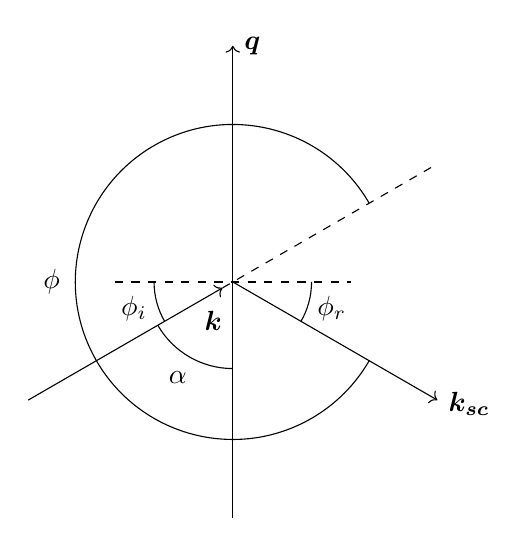
\begin{tikzpicture}

	% Draw wave vectors
	\draw[->] (0,-3) -- (0,3);
	\draw[->,rotate=30] (-3,0) -- (-0.15,0);
	\draw[->,rotate=-30] (0,0) -- (3,0);
	\draw (3,-1.55) node{$\bm{k_\mrm{sc}}$} (0.25,3) node{$\bm{q}$} (-0.25,-0.5) node{$\bm{k}$};
	
	% Draw dashed lines
	\draw[dashed,rotate=30] (-0.15,0) -- (3,0);
	\draw[dashed] (-1.5,0) -- (1.5,0);
	
	% Draw angles
	\draw ([shift={(30:2)}] 0,0) arc(30:330:2) (180:2.3) node{$\phi$};
	\draw ([shift={(-150:1.1)}] 0,0) arc(-150:-90:1.1) (-120:1.4) node{$\alpha$};
	\draw ([shift={(180:1)}] 0,0) arc(180:210:1) (195:1.3) node{$\phi_\mrm{i}$};
	\draw ([shift={(0:1)}] 0,0) arc(0:-30:1) (-15:1.3) node{$\phi_\mrm{r}$};
	
\end{tikzpicture}
			\caption{- case}
		\end{subfigure}
		\caption{\label{fig:bragg-comparison} Comparison of angles used in this model and angles of incidence and reflection. Both for the + and - cases.}
	\end{figure}

\subsection{Refined interaction region}
For the refined interaction region described in section \ref{sec:app-derivations-refined} the derivation for finding a maximum scattering geometry is different than above. However, a first hypothesis would be that the resulting condition would be the same. To test this, the angles described by equations \eqref{eq:app-bragg-theta}, \eqref{eq:app-bragg-alpha}, \eqref{eq:app-bragg-phi} are inserted in $\Phi_p^{\pm}(\theta, \phi)$ from section \ref{sec:app-derivations-refined}. The function can be written as
\begin{equation*}
\begin{split}
	\Phi_p^{\pm}(\theta, \phi) &= \text{sinc}\left( \frac{d_a}{2\pi \sin{\alpha}}(k - k\sin{\theta}\cos{\phi} \pm q\cos{\alpha}) \right) \\
	&\cdot \text{sinc}\left( \frac{d_e}{2\pi \tan{\alpha}}
	(k - k\sin{\theta}(\cos{\phi} + \sin{\phi}\tan{\alpha}) \pm q(\cos{\alpha} + \sin{\alpha}\tan{\alpha})) \right) \\
	&\cdot \text{sinc}\left( -\frac{L_z}{2\pi} k\cos{\theta} \right)
\end{split}
\end{equation*}
As for the function used in derivations for the cuboid geometry, the maximum value of this function is 1. This happens only when the arguments of all sinc's are 0. Due to this fact, the problem is simplified by only considering the parts of the arguments required to be zero, namely
\begin{numcases}{}
	k - k\sin{\theta}\cos{\phi} \pm q\cos{\alpha} \label{eq:app-bragg-ref1} \\
	k - k\sin{\theta}(\cos{\phi} + \sin{\phi}\tan{\alpha}) \pm q(\cos{\alpha} + \sin{\alpha}\tan{\alpha} \label{eq:app-bragg-ref2} \\
	-\frac{L_z}{2\pi} k\cos{\theta} \label{eq:app-bragg-ref3}
\end{numcases}
Now the equations \eqref{eq:app-bragg-theta}, \eqref{eq:app-bragg-alpha}, \eqref{eq:app-bragg-phi} are inserted. In the derivations the following relations are well used
\begin{align*}
	\cos(\mp \pi + 2\alpha) &= \sin^2{\alpha} - \cos^2{\alpha} \\
	\sin(\mp \pi + 2\alpha) &= -2\sin{\alpha}\cos{\alpha} \\
	q &= \mp 2k\cos{\alpha}
\end{align*}
Argument \eqref{eq:app-bragg-ref1} is now written as
\begin{equation*}
\begin{split}
	k &- k\sin(\pi/2)\cos(\mp \pi + 2\alpha) \pm q\cos{\alpha} = k \left( 1 - (\sin^2{\alpha} - \cos^2{\alpha}) \pm (\mp 2\cos^2{\alpha}) \right) \\
	&= k \left( 1 - \sin^2{\alpha} - \cos^2{\alpha} \right) = 0
\end{split}
\end{equation*}
Since it is equal to zero, the first sinc is maximized. Now argument \eqref{eq:app-bragg-ref2} is written as
\begin{equation*}
\begin{split}
	k &- k\sin(\pi/2)(\cos(\mp \pi + 2\alpha) + \sin(\mp \pi + 2\alpha)\tan{\alpha}) \pm q(\cos{\alpha} + \sin{\alpha}\tan{\alpha} \\
	&= k \left( 1 - (\sin^2{\alpha} - \cos^2{\alpha} - 2\sin{\alpha}\cos{\alpha}\tan{\alpha}) \pm (\mp 2\cos{\alpha})(\cos{\alpha} + \sin{\alpha}\tan{\alpha}) \right) \\
	&= k \left( 1 - \sin^2{\alpha} + \cos^2{\alpha} + 2\sin^2{\alpha} - 2\cos^2{\alpha} - 2\sin^2{\alpha} \right) \\
	&= k \left( 1 - \sin^2{\alpha} - \cos^2{\alpha} \right) = 0
\end{split}
\end{equation*}
Since it is equal to zero, the second sinc is maximized. Finally, argument \eqref{eq:app-bragg-ref3} is written as
\begin{equation*}
	-\frac{L_z}{2\pi} k\cos{\pi/2} = 0
\end{equation*}
Since it is equal to zero, the third sinc is also maximized. Thus, all sinc functions are maximized which maximizes $\Phi_p^{\pm}$. This shows that the same condition (equations \eqref{eq:app-bragg-theta}, \eqref{eq:app-bragg-alpha}, \eqref{eq:app-bragg-phi}) maximizes the scattering for both the simple cuboid geometry and the refined geometry based on beams.
\todoint[inline]{Explain factor 1/sin(alpha) related to scattering volume and why this is not included in the maximization thing}
	
\end{document}